
\documentclass[12pt]{article}
\usepackage[T1]{fontenc}
\usepackage{hyperref}
\usepackage{amsmath}
\usepackage{graphicx}
\usepackage{tikz, mhchem}
\usepackage{mathtools}
\usepackage[section]{placeins}
\usepackage{float}% If comment this, figure moves to Page 2


\setcounter{figure}{0}

\title{Free Amino Acids in Human Milk: Time and Infant Gender}
\author{Federico J. Zertuche}
\date{\today}

\begin{document}
\maketitle

\begin{abstract}
This report has the objective of comparing our results with those in the litterature, specifically those found here:

\begin{center}
  \href{https://www.mdpi.com/2072-6643/10/9/1233}{https://www.mdpi.com/2072-6643/10/9/1233}
\end{center}

It is divided into $3$ parts:

The first is about understanding the data. I try to describe and motivate the models, significant results and thier relationship with existing literature and medical knowledge.

In the second, the models are used to understand what should we be looking forward to in future experiments. Here, I take the models seriously and device possible predictions that are compatible with current knowledge.

The third part is about missing data. I mention what I did with the missing patients.

\end{abstract}

\part{Three Objectives, Three Models}

I am interested in answering $3$ questions:

\begin{enumerate}
  \item Do amino acid levels change over time?
  \item Are these levels different in the milk for boys and girls?
  \item If the concentration changes over time, is it different for boys and girls?
\end{enumerate}

I use $3$ regression models to summarize the effects for each one of the questions. The answers are given as coefficients with confidence intervlas.

Before analyzing the results let me introduce some notation.

I will write $AA$ for the concentration level of a particular amino acid. The data contains the concentration of several amino acids. In general, I will study them individually. I use the essential and non essential classification since I am interested in the difference between nourishment and body production.

The measurements were taken at weeks $1, 2, 8$ and $16$ so the variable corresponding to time is called $week$. This is not a categorical variable.

I note the infant genders $boy$ and $girl$ and the variable will be called $sex$.

There is an additional variable called $group$ that tells us if the mother was a $teen$ or an $adult$ when she gave birth.

\section{Do AA levels change over time?}

Here the model used is:

\begin{equation} \label{eq:model1}
  AA = \alpha_0 + \alpha_1 \ week + \alpha_{id}
\end{equation}

Each coefficient is the summary of an effect.

The first, $\alpha_0$, is the concentration at week $0$, I will not talk about this coefficient. The second one has units $concentration/time$, it is the main focus in this part of the analysis.

The last one represents a random effect that is different for each one of the participats, think about it as all the patients differences that were not controlled for during the data collection process.

\subsection{Essential Amino Acids}

\begin{figure}[!htb]
  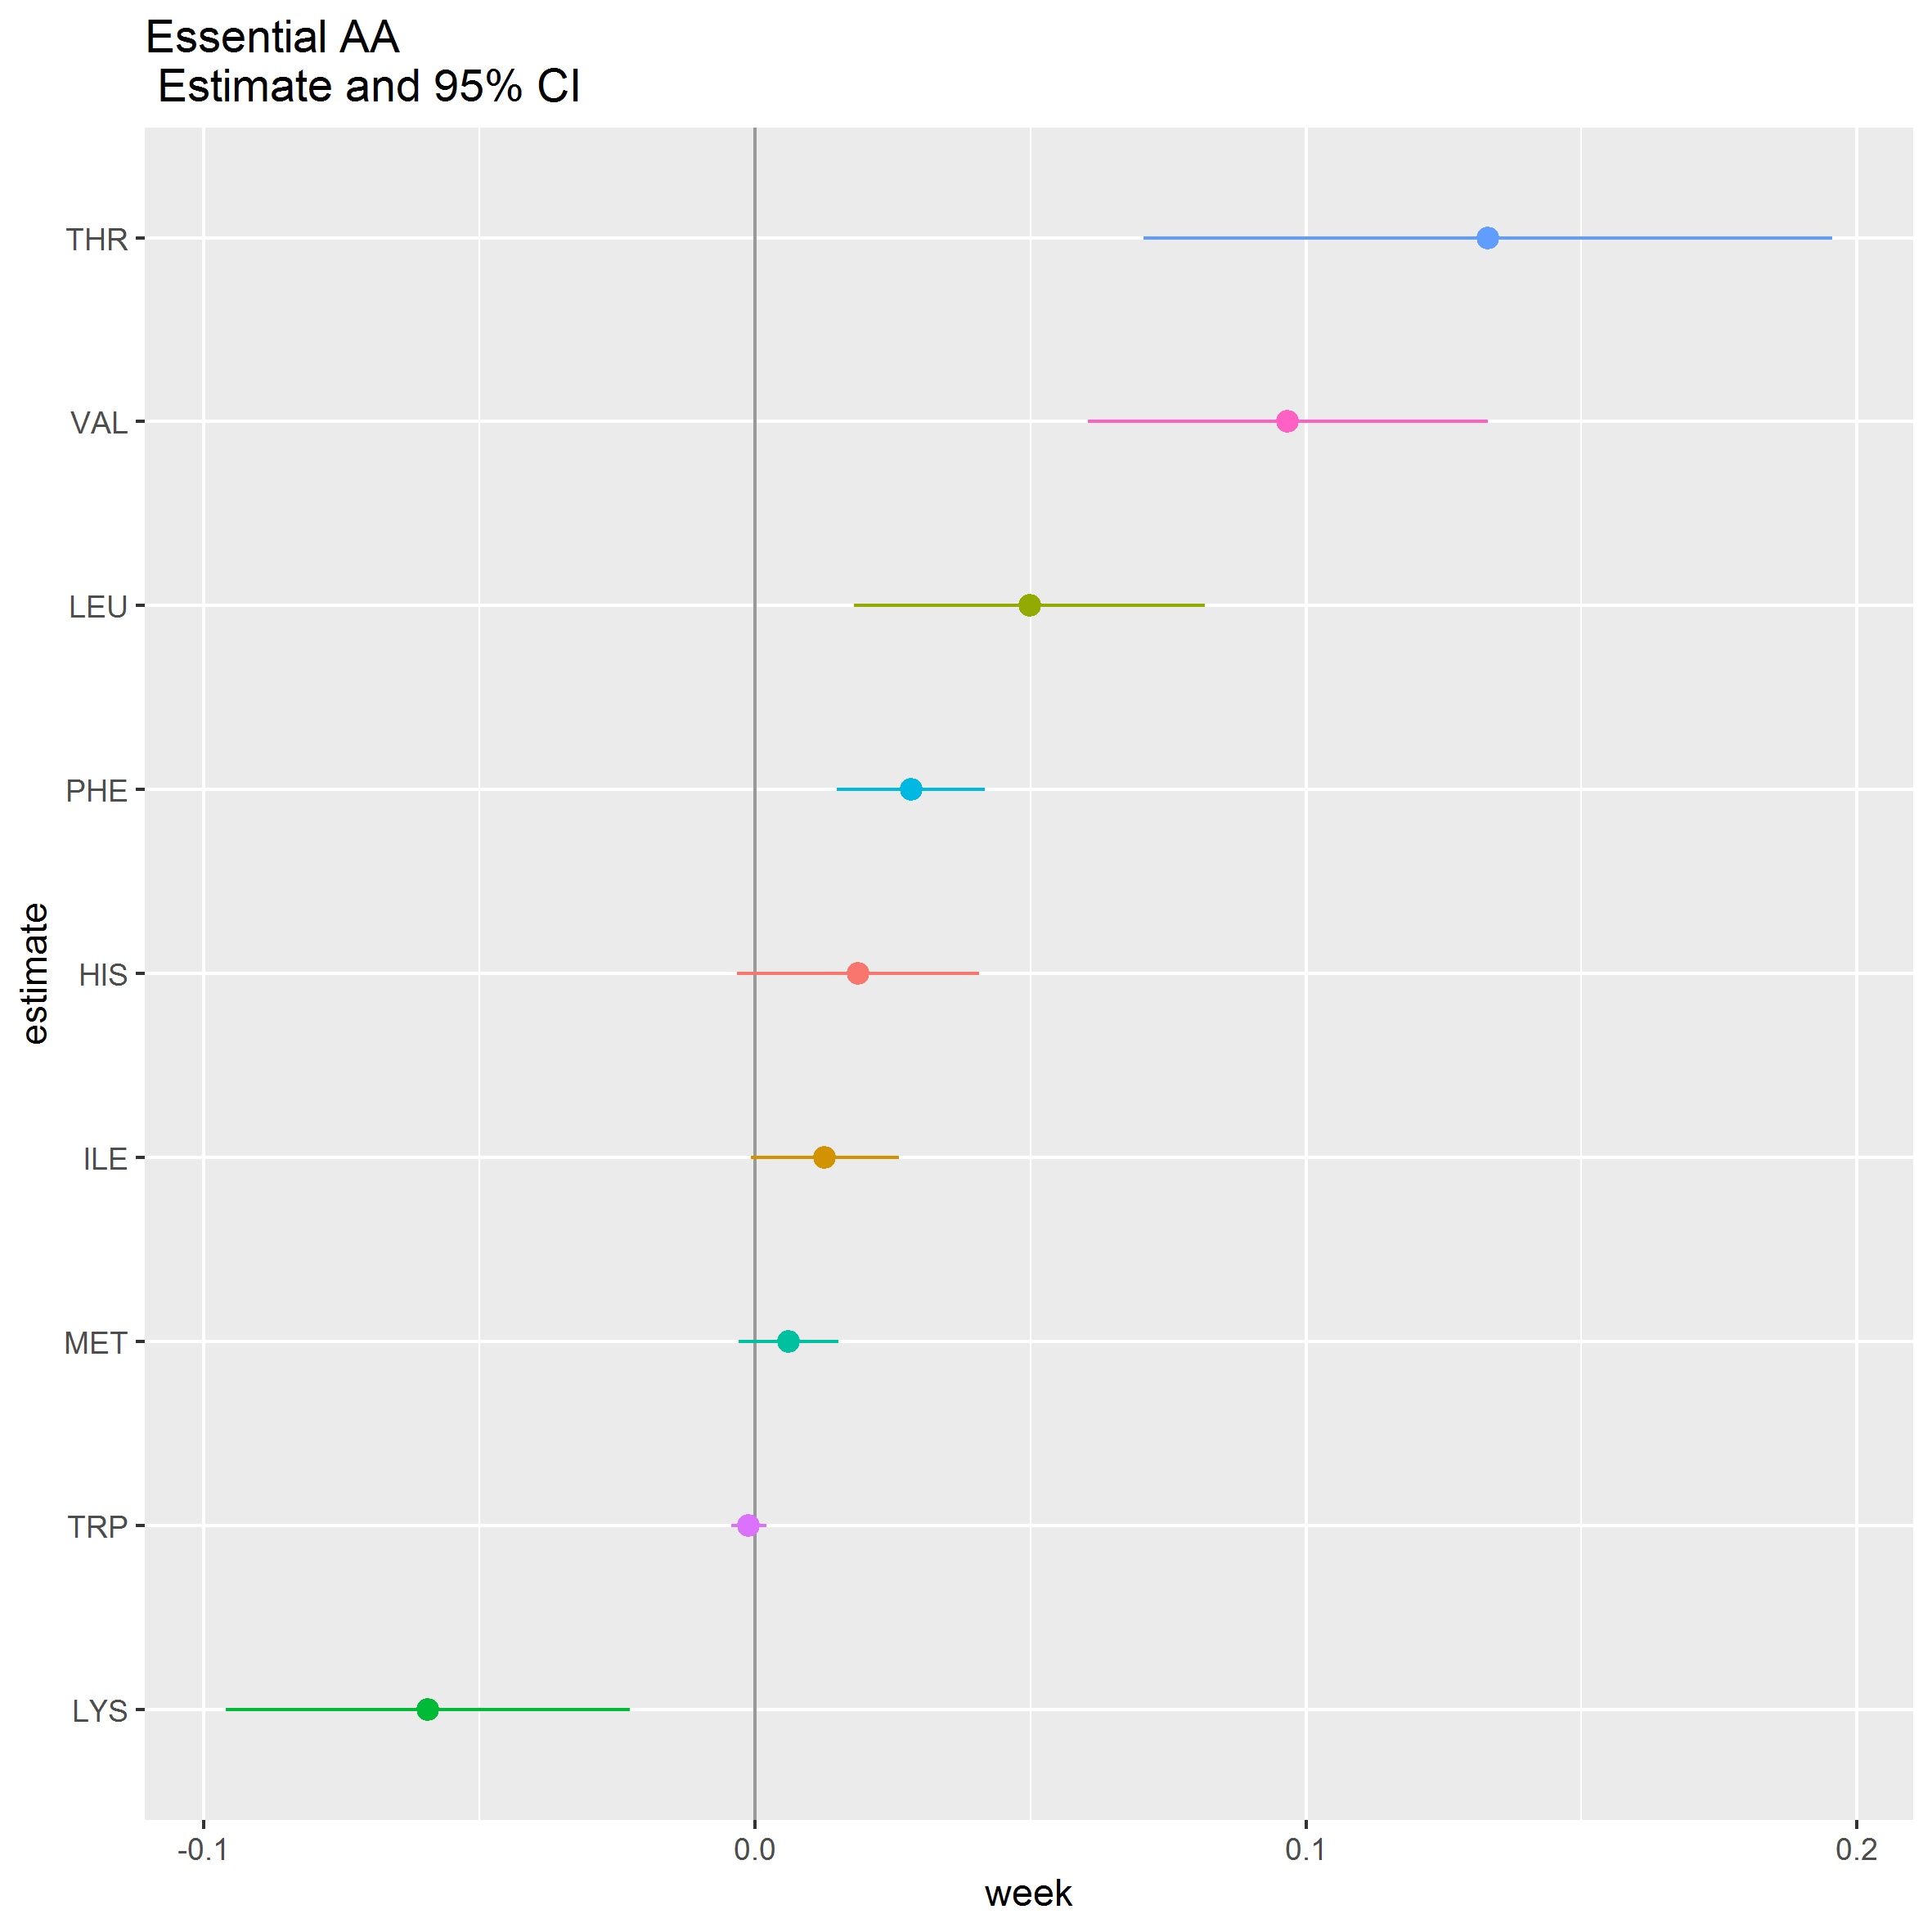
\includegraphics[width= \textwidth]{../week/EAA_W_coeff.png}
  \caption{Week coefficients of model (\ref{eq:model1}) for essential amino acids.}
  \label{fig:EAA_W_coeff}
\end{figure}

The list of amino acids with significant effects (figure \ref{fig:EAA_W_coeff}) over time is: THR, VAL, LUE, PHE. As you can see in figure \ref{fig:EAA_simple}, in all of these amino acids, there a is general increasing or decresing trend. The coefficients are meant to capture this. This model does not capture phenomena like the decrease from week $8$ to $16$ in PHE and VAL. Think of the model as a first approximation that helps us with calssifying the concentrations.

\begin{figure}[!htb]
  \centering
  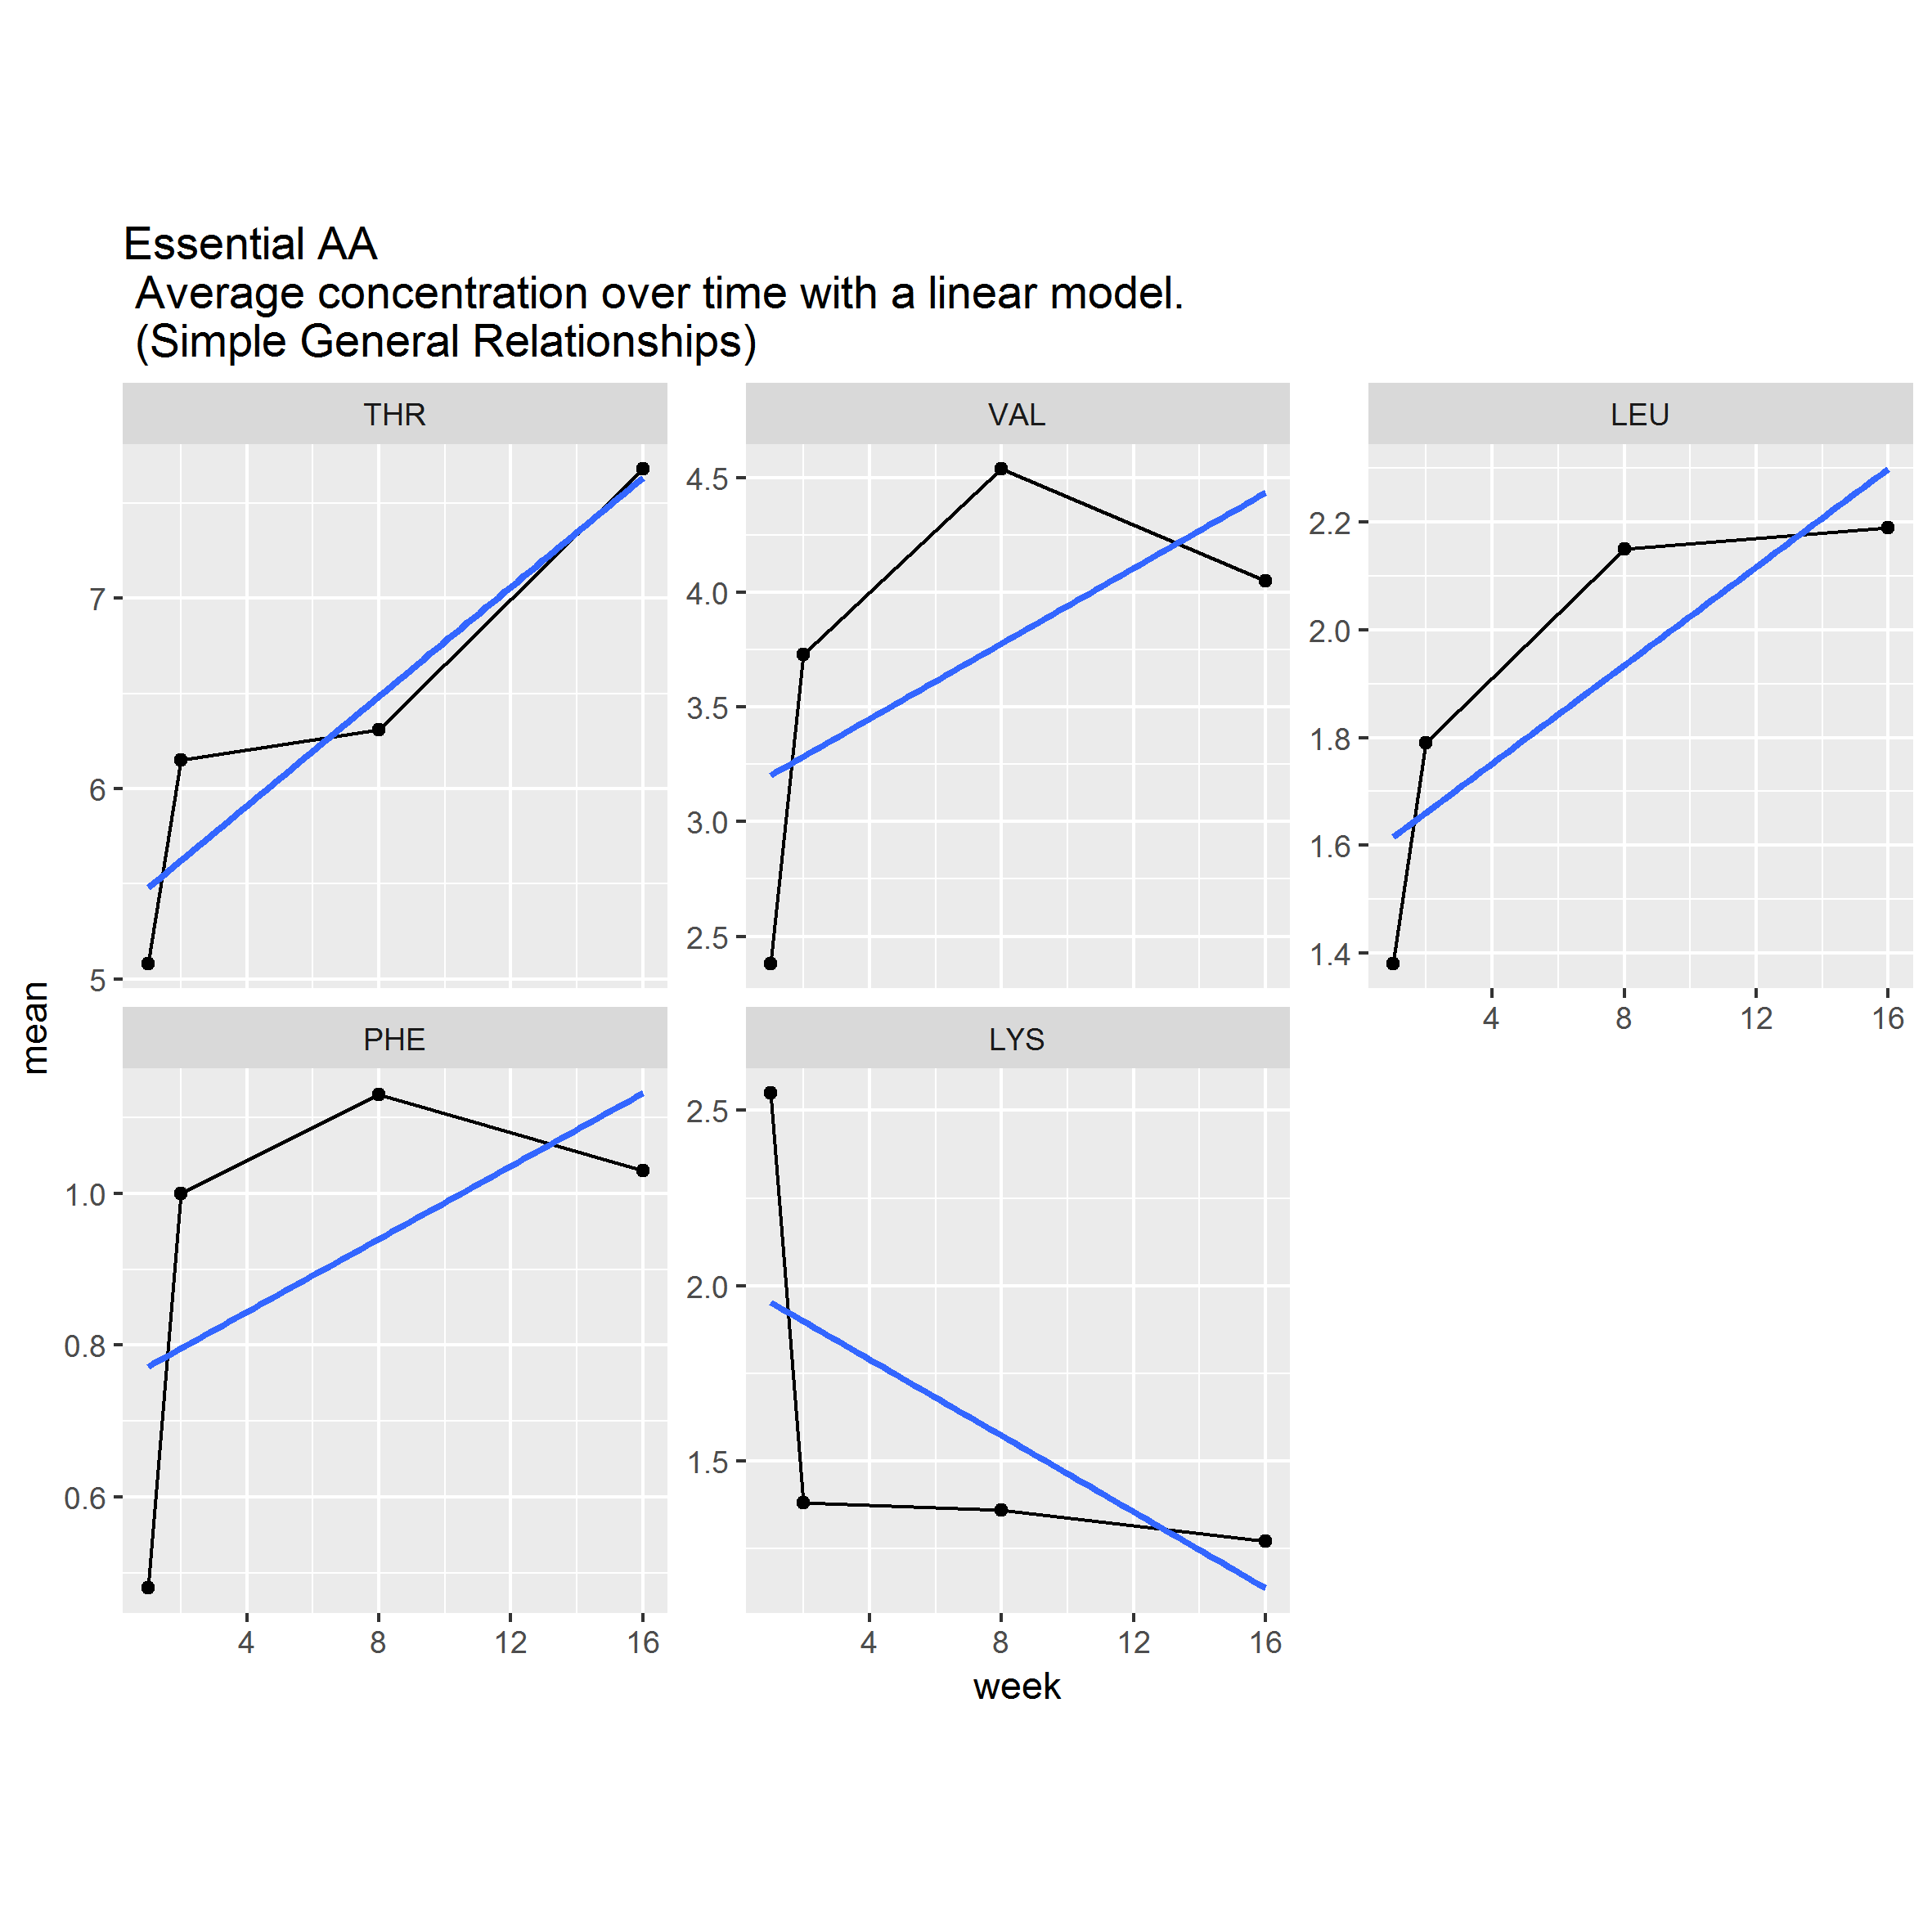
\includegraphics[width=\textwidth]{../week/EAA_simple.png}
  \caption{Mean concentration per week with a linear regression line in blue. Essential amino acids with significant week effects.}
  \label{fig:EAA_simple}
\end{figure}


Four amino acids have non significant effects: HIS, ILE, MET and TRP. Figure \ref{fig:EAA_complex} shows their mean concentration over time. In each of the figures there is an abrupt change. For example, TRP jumps between positive and zero concentrations, probably due to the size of the measurements (the highest vaule is $0.03$). In ILE and MET there is an abrupt decrease from month $8$ to $16$. Finally, HIS has a big increase from week $1$ to $2$ and a steady decrease from there on. Once again, all these non linear patterns are not very well described by model (\ref{eq:model1}).

\begin{figure}[!htb]
  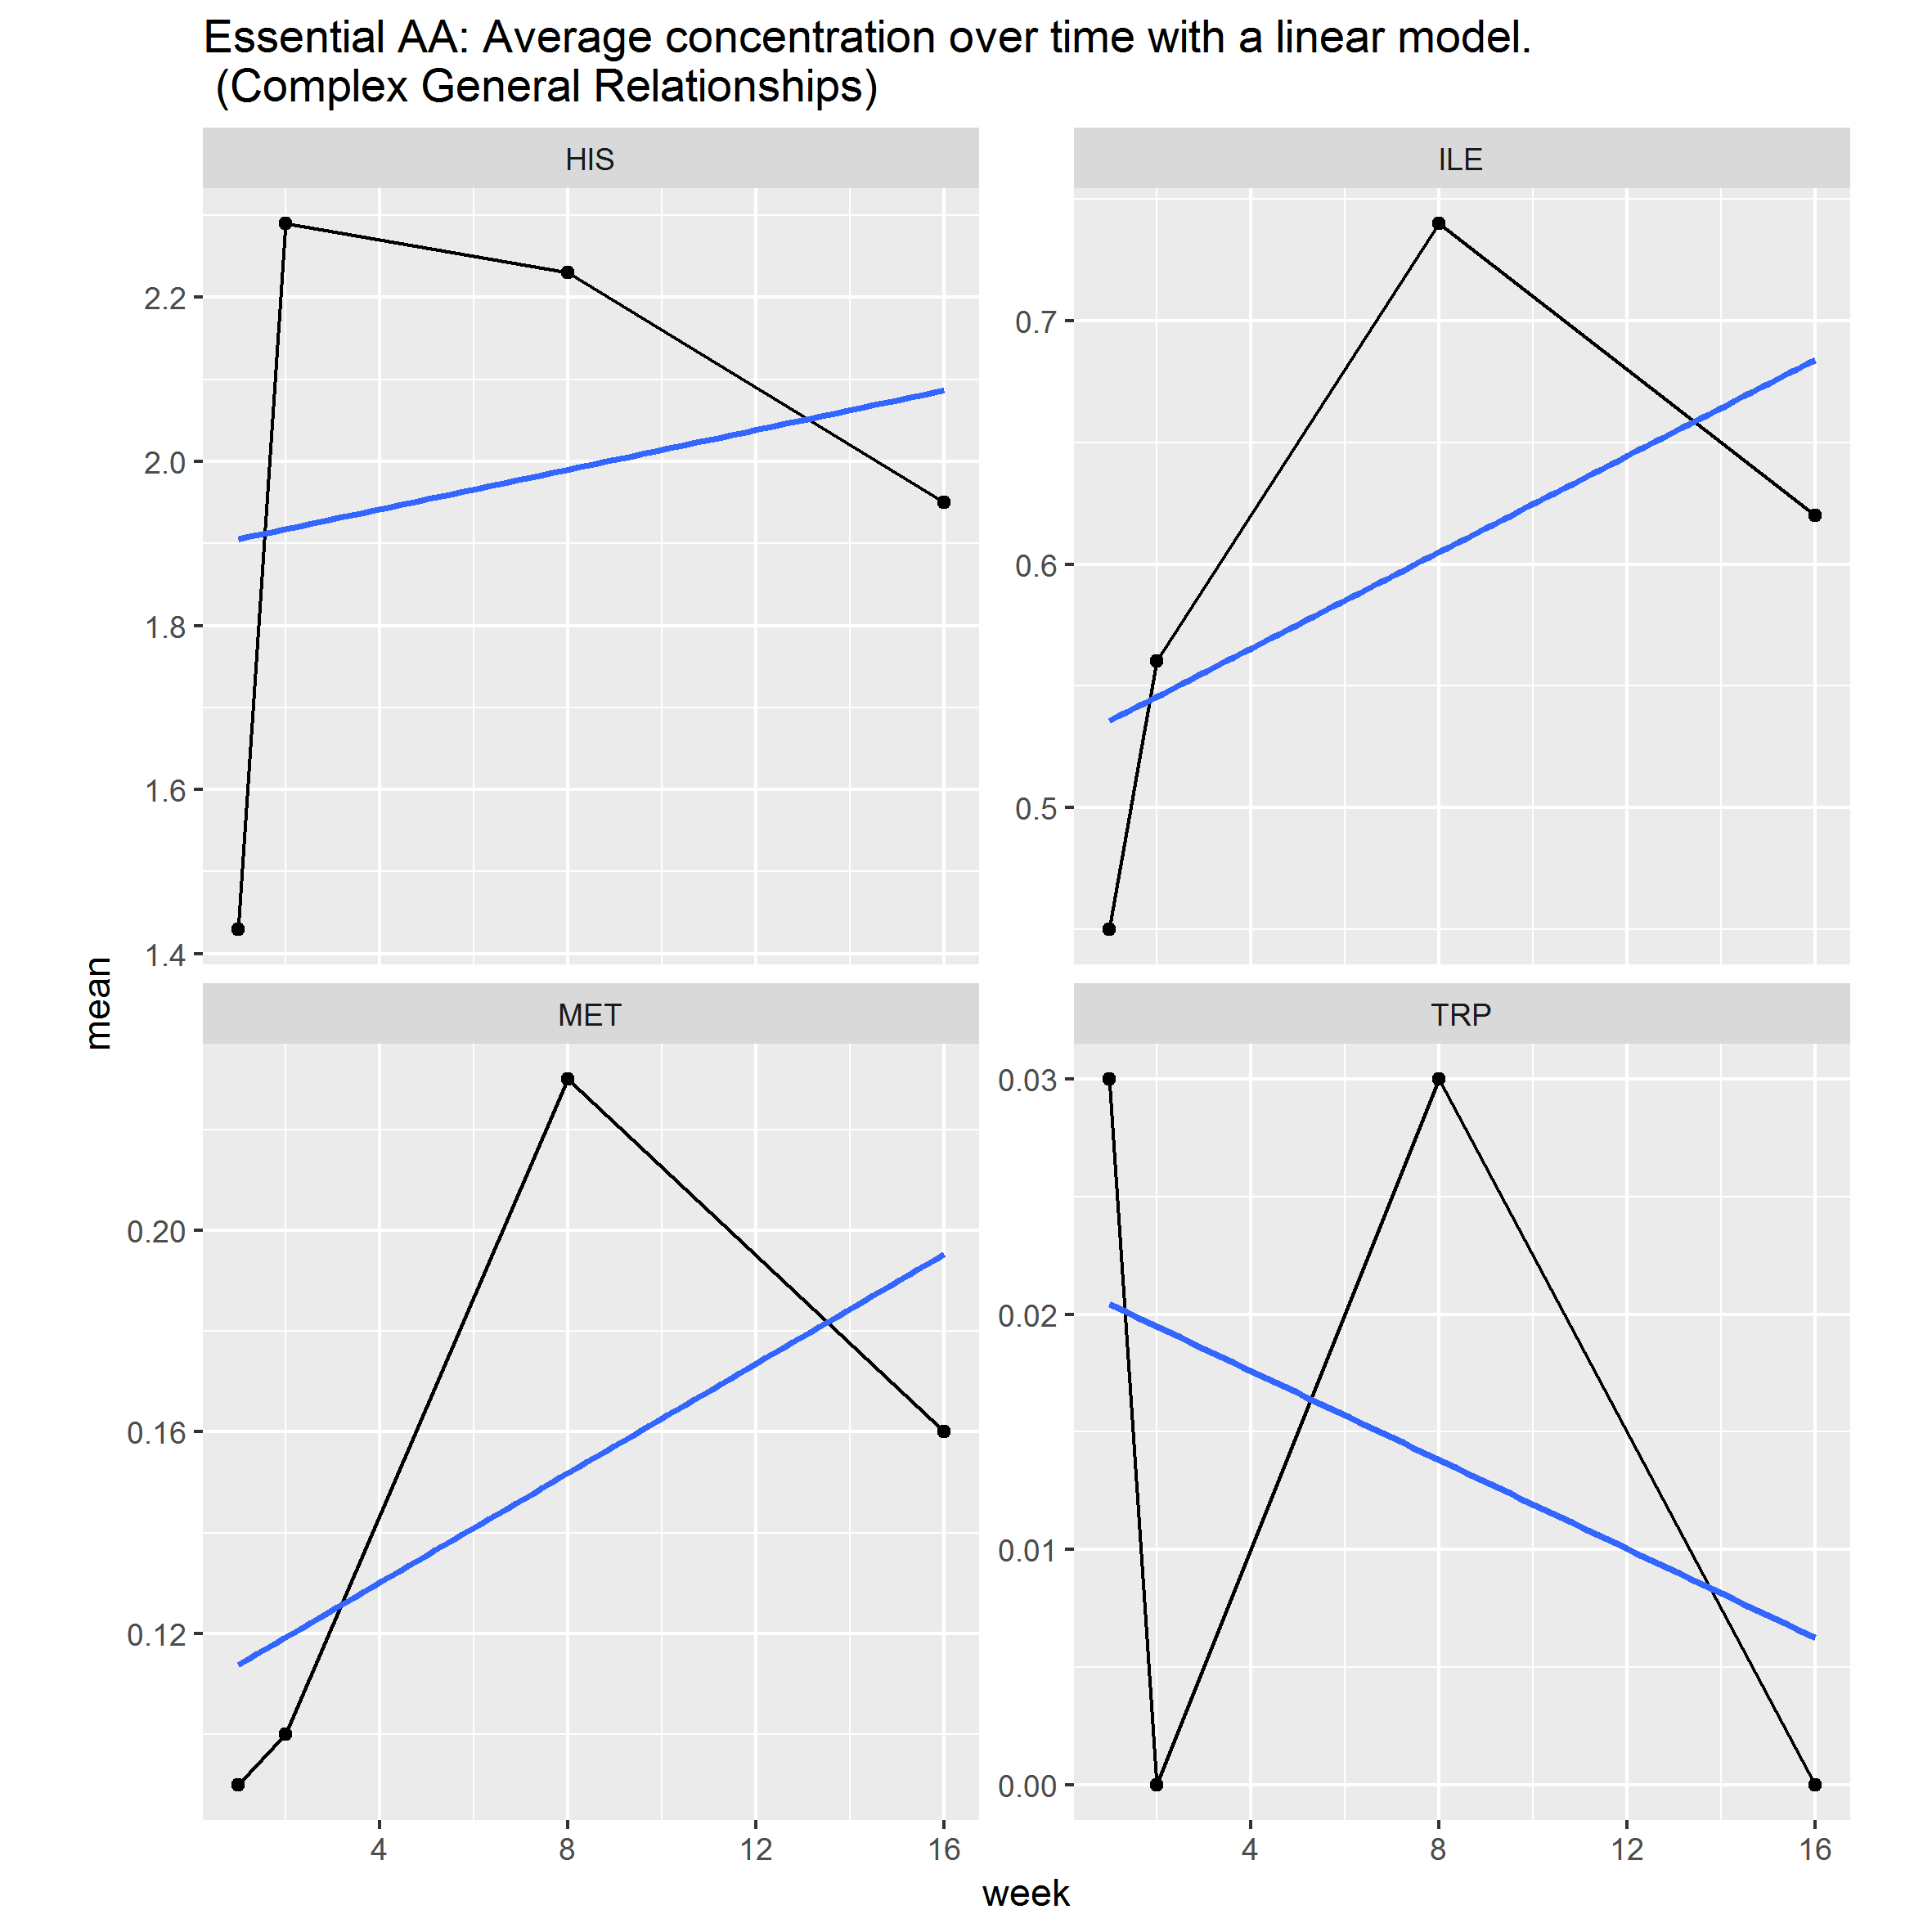
\includegraphics[width= \textwidth]{../week/EAA_complex.png}
  \caption{Mean concentration per week with a linear regression line in blue. Essential amino acids with non significant week effects.}
  \label{fig:EAA_complex}
\end{figure}

\subsection{Non Essential Amino Acids}

The effects for the non essential amino acids are shown in figure \ref{fig:NEAA_W_coeff}. Figure \ref{fig:NEAA_W_coeff_detail} shows the small coeffients in detail.

The concentrations of $ARG$ and $PRO$, in figure \ref{fig:NEAA_simple}, decrease in a similar pattern as that of LYS in figure \ref{fig:EAA_simple}. First a big drop from week $1$ to $2$ and a slower decrease afterwards.

All the other significant effects are positive, the concentration of GLU, GLN, ALA, SER, GLY, ASP, CYS and TYR increases over time as shown in figure \ref{fig:NEAA_simple}.

The only non significant effect is that of ASN. Figure \ref{fig:NEAA_complex} shows how its concentration changes over time: first a big drop and then a big increase. Studying what happens between weeks $2$ and $8$ might help in understanding how this concentration varies over time.

\begin{figure}[!htb]
  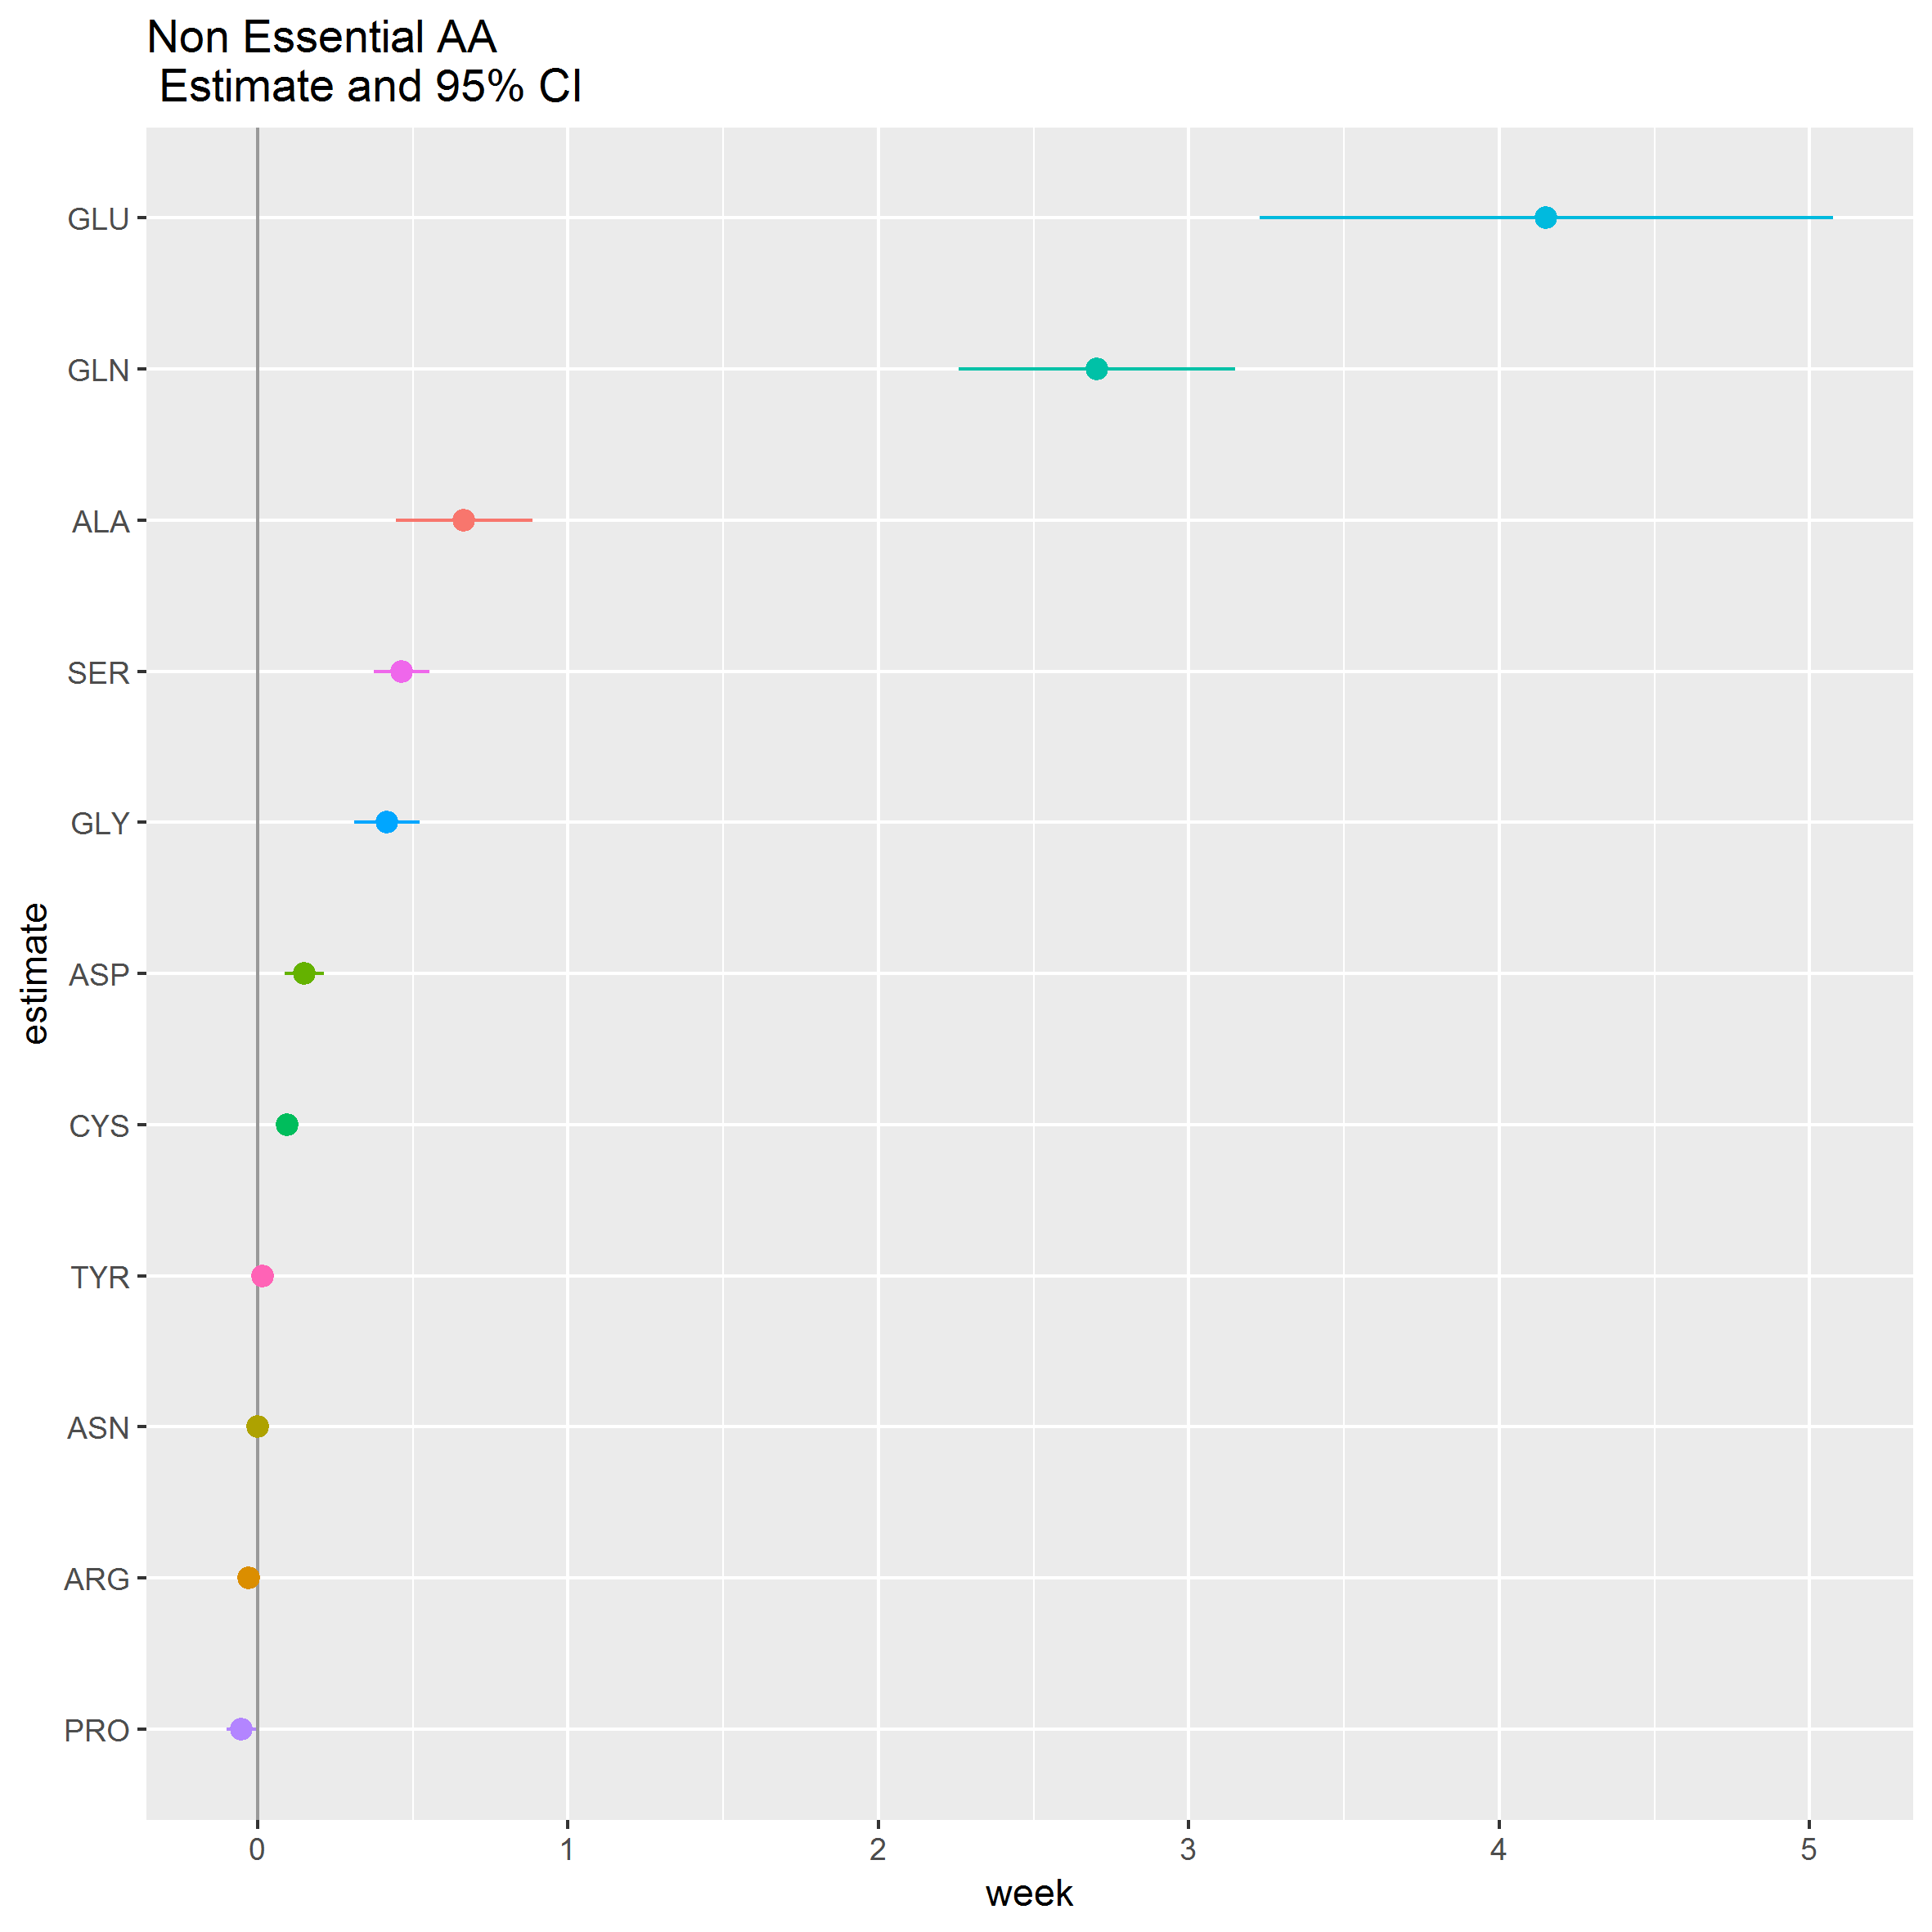
\includegraphics[width= \textwidth]{../week/NEAA_W_coeff.png}
  \caption{Week coefficients of model (\ref{eq:model1}) for non essential amino acids.}
  \label{fig:NEAA_W_coeff}
\end{figure}

\begin{figure}[!htb]
  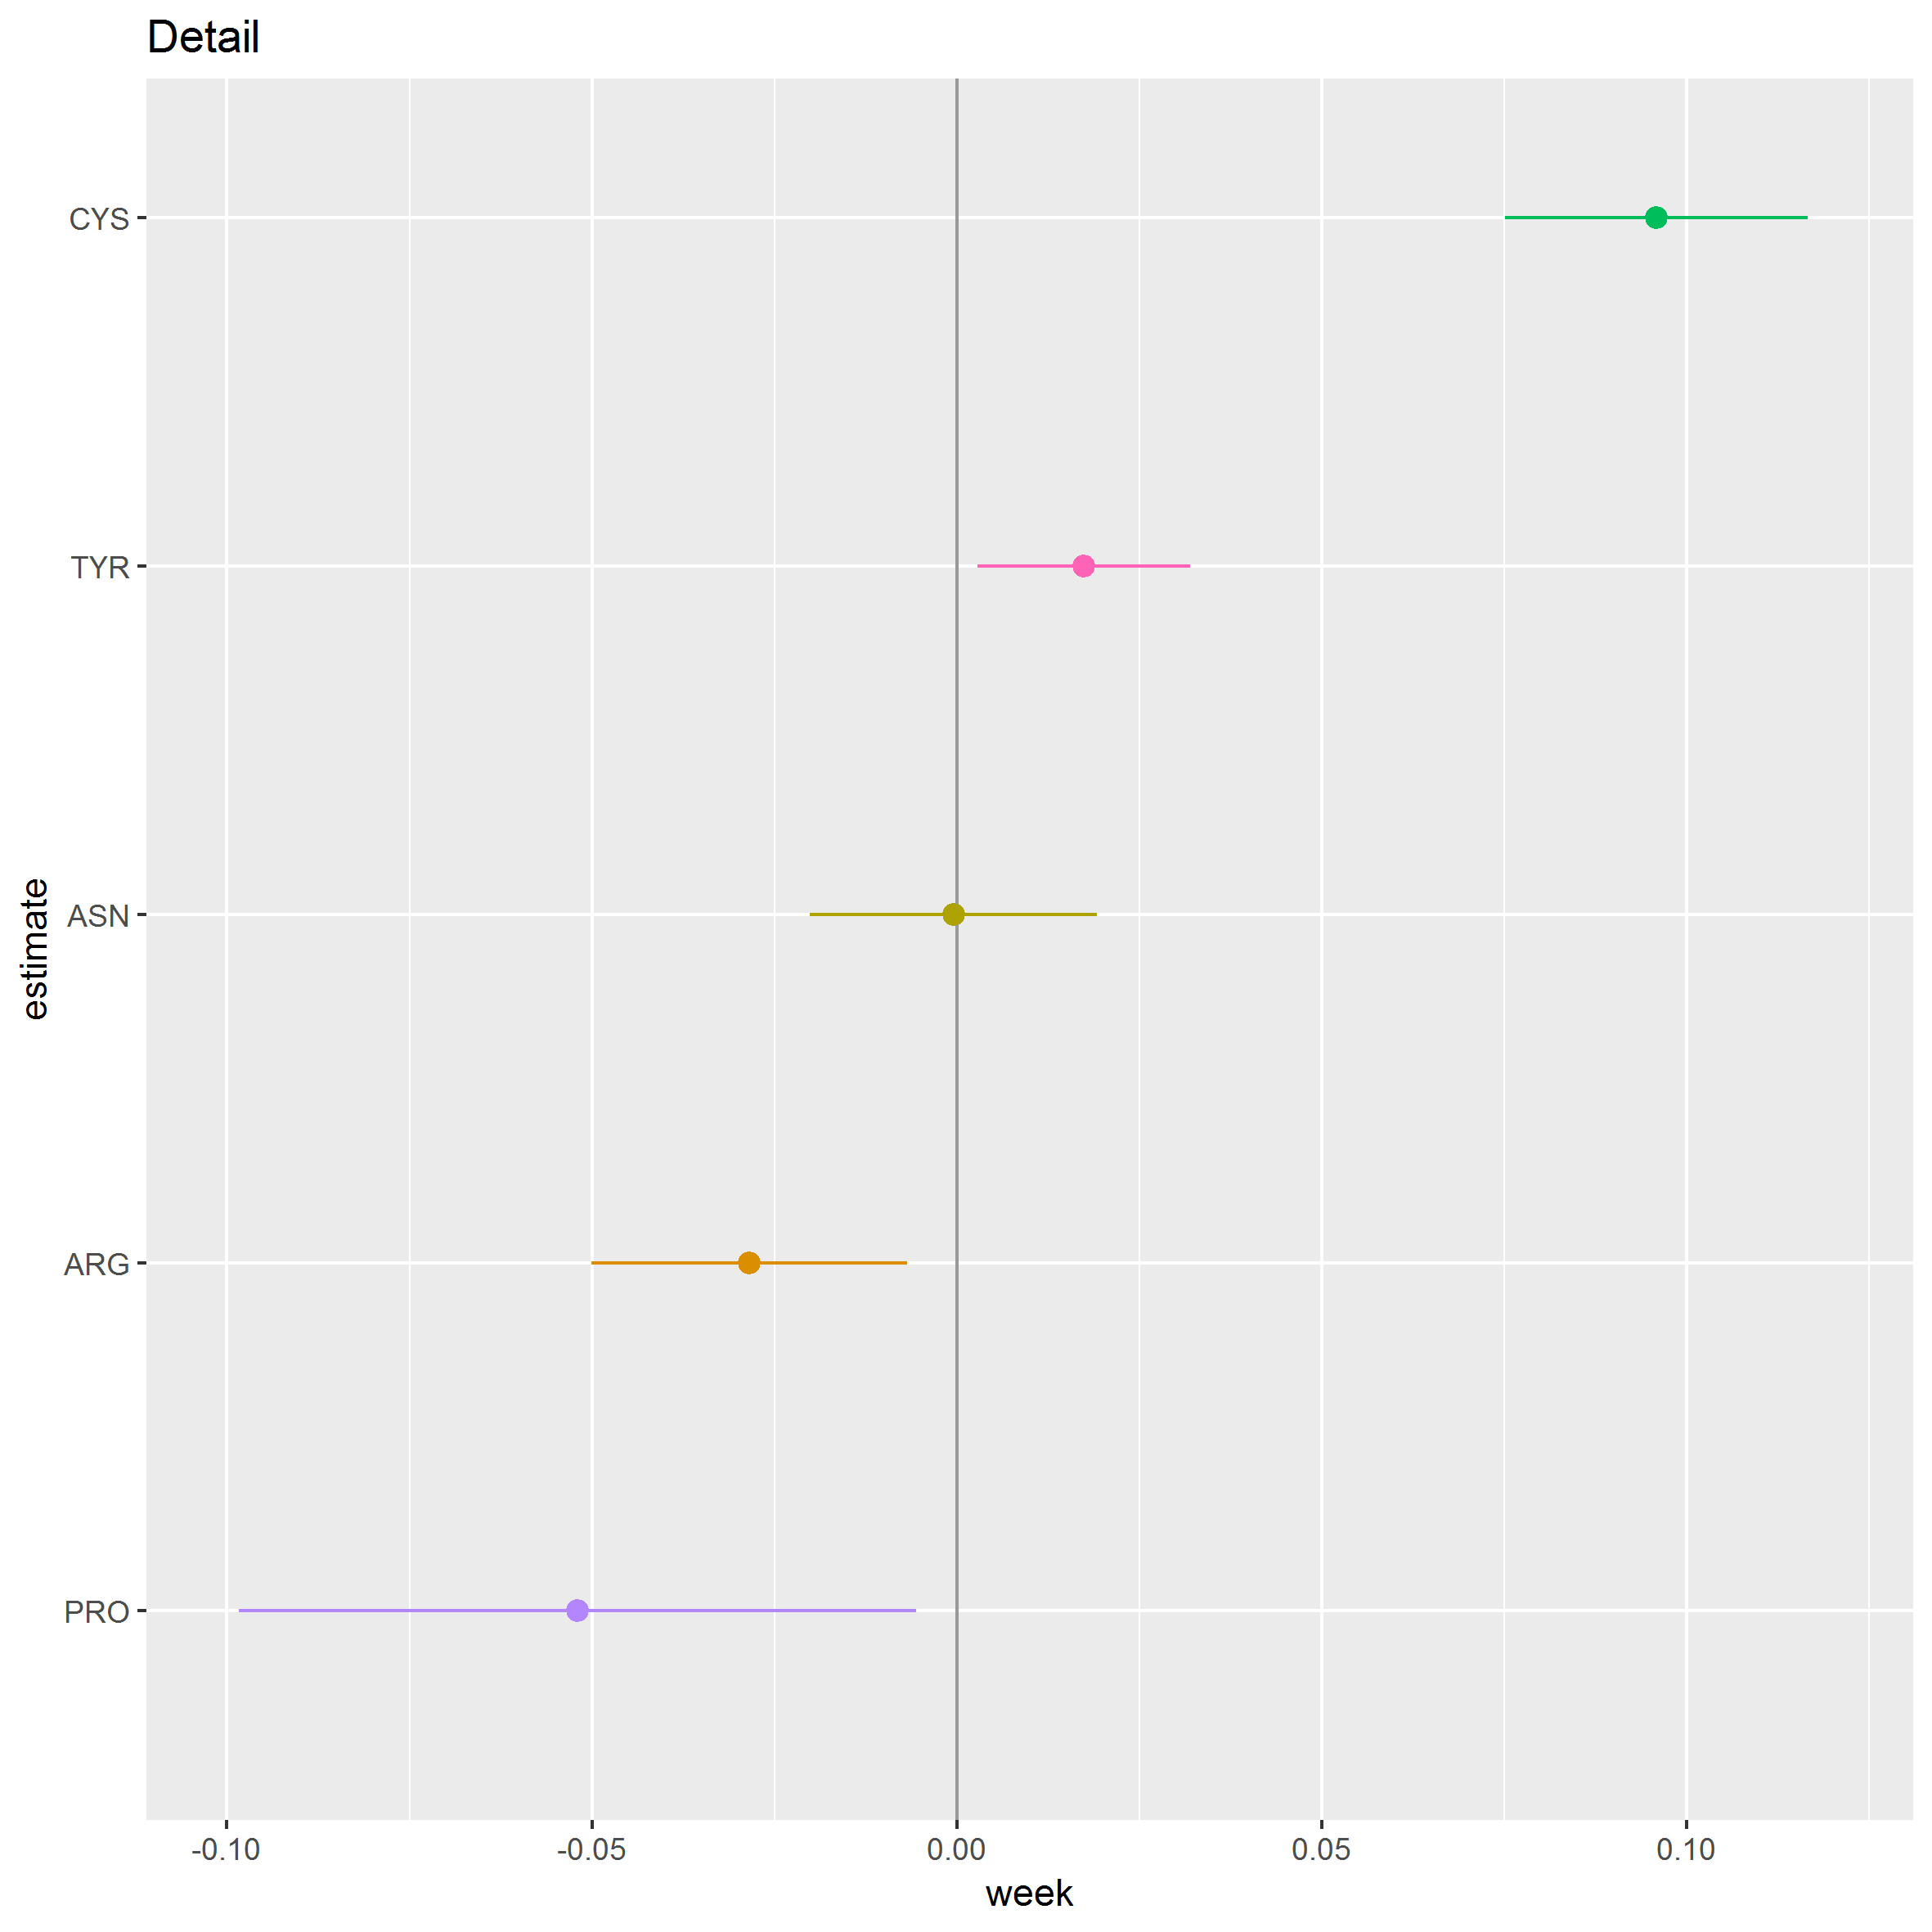
\includegraphics[width= \textwidth]{../week/NEAA_W_coeff_detail.png}
  \caption{Detail of the week coefficients of model (\ref{eq:model1}) for the non essential amino acids with small effects.}
  \label{fig:NEAA_W_coeff_detail}
\end{figure}

\begin{figure}[!htb]
  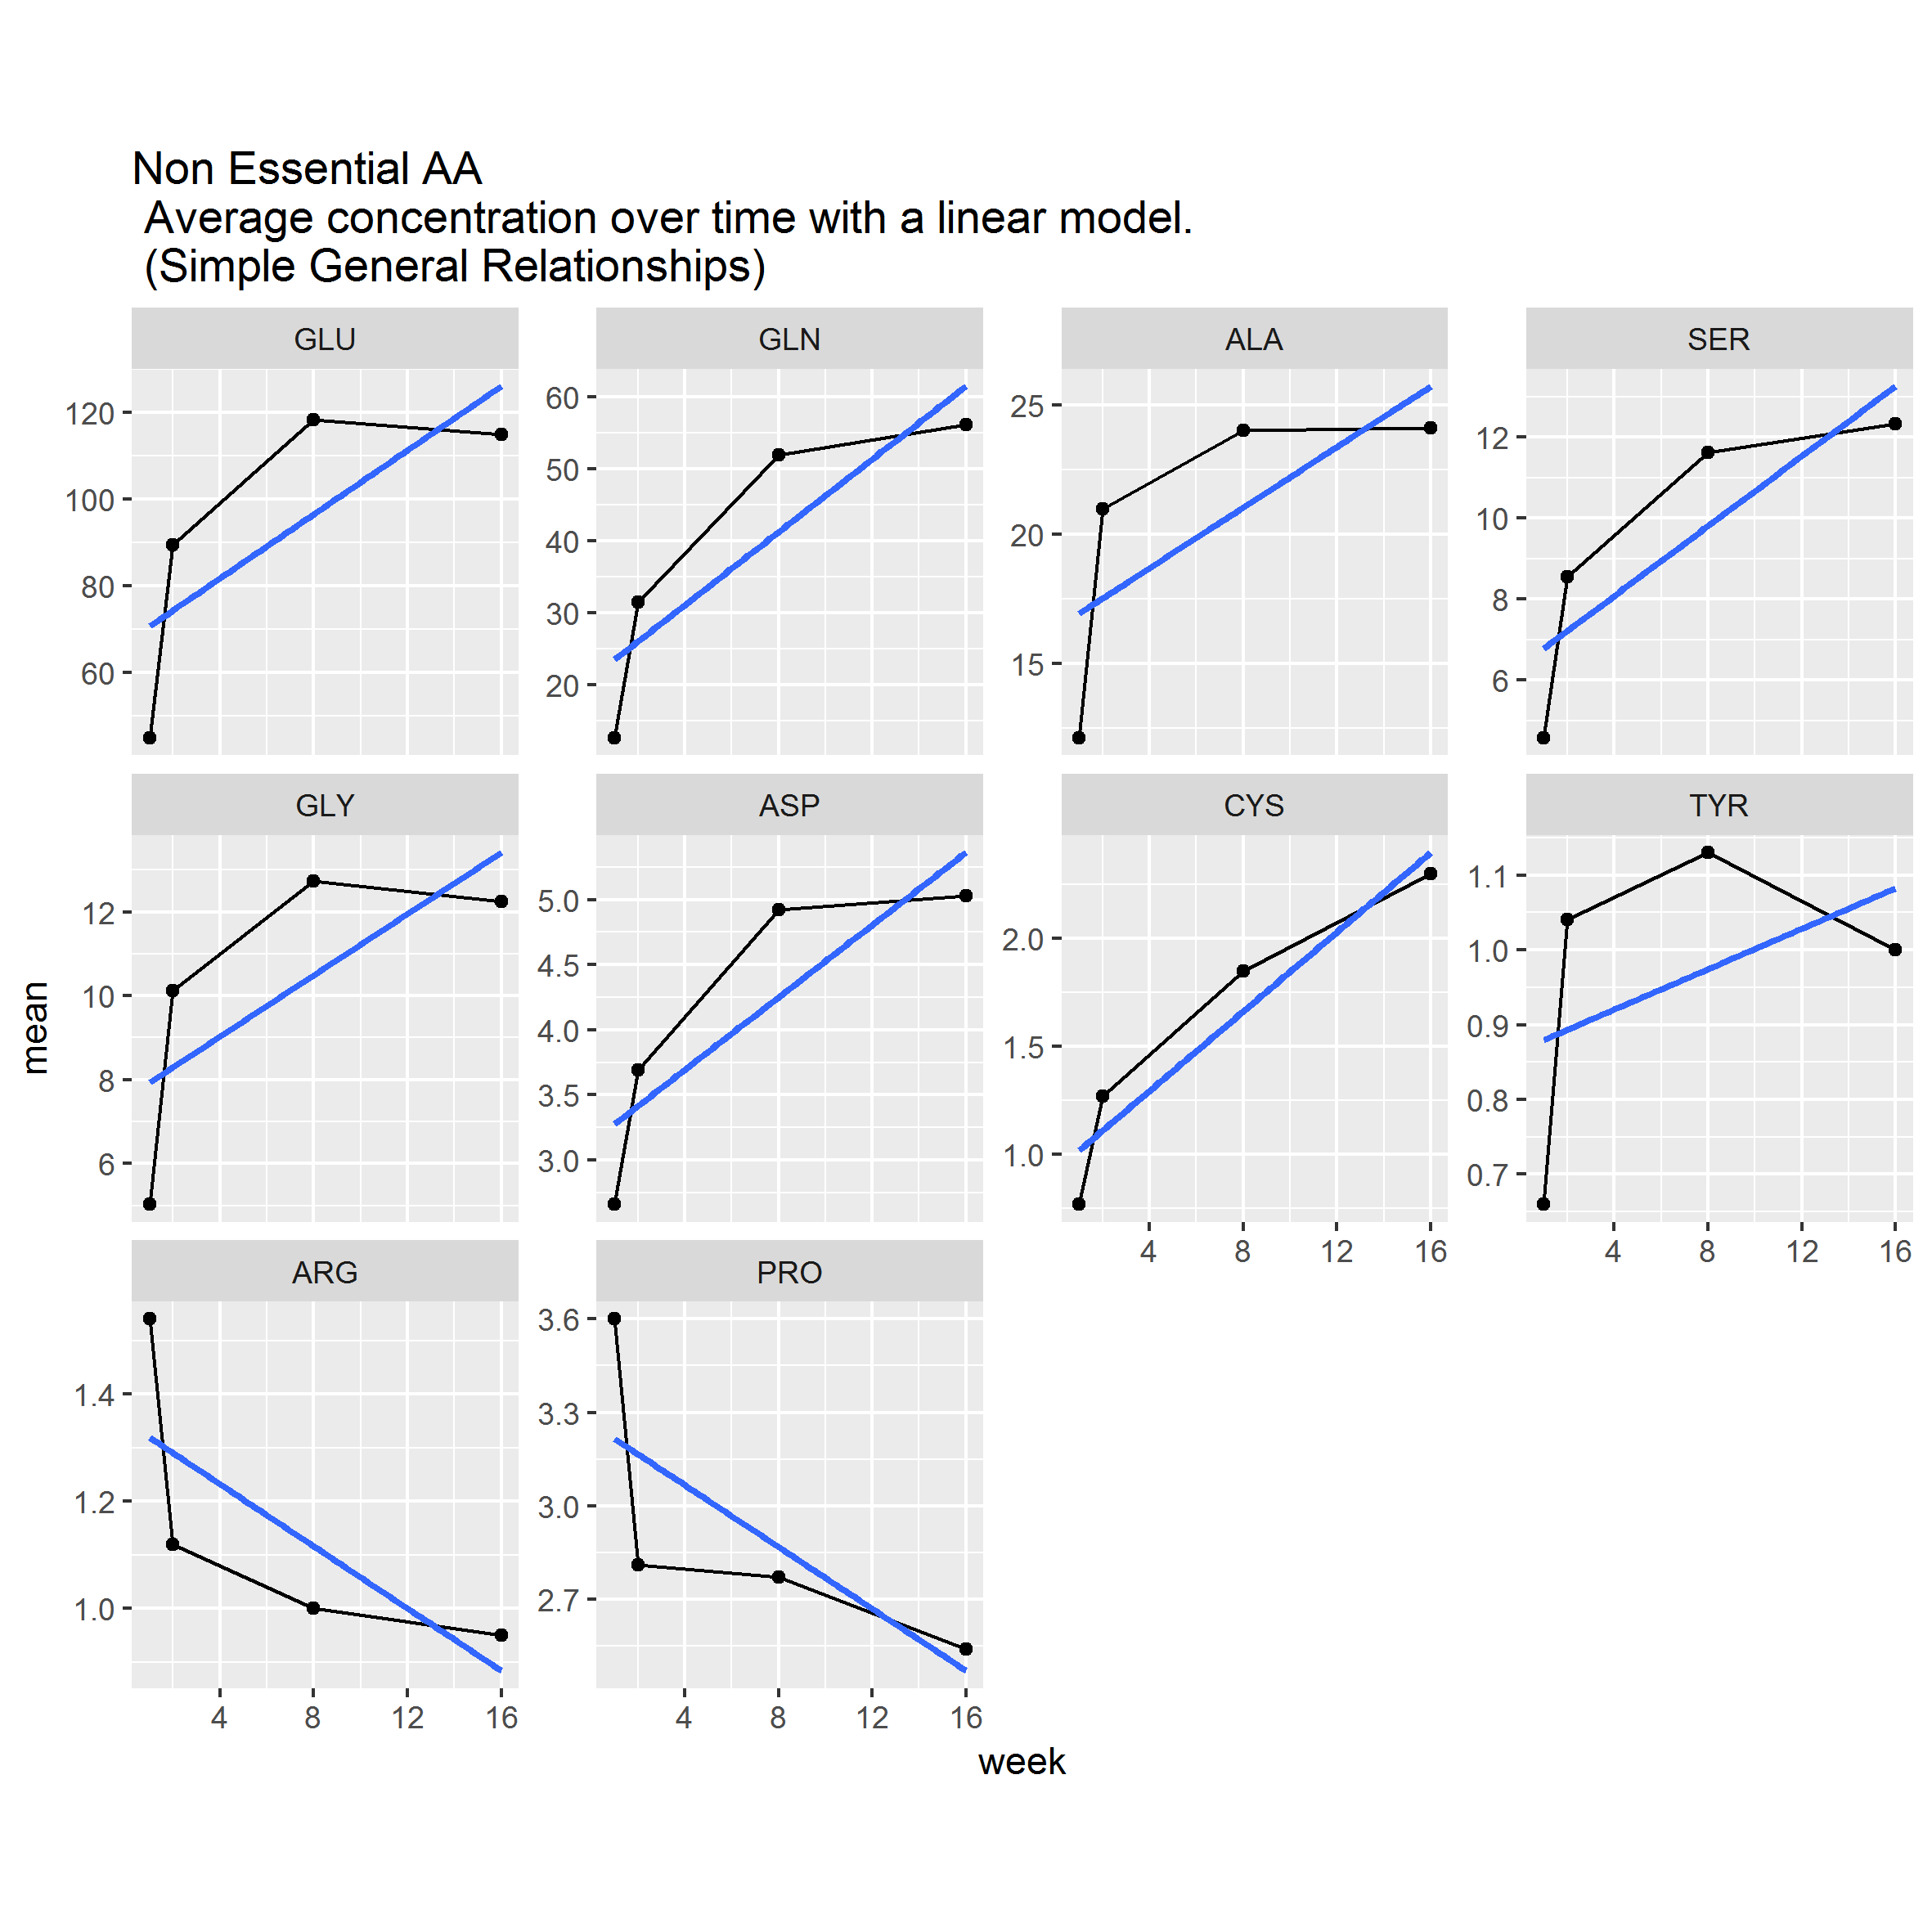
\includegraphics[width= \textwidth]{../week/NEAA_simple.png}
  \caption{Mean concentration per week with a linear regression line in blue. Non essential amino acids with significant week effects.}
  \label{fig:NEAA_simple}
\end{figure}

\begin{figure}[!htb]
  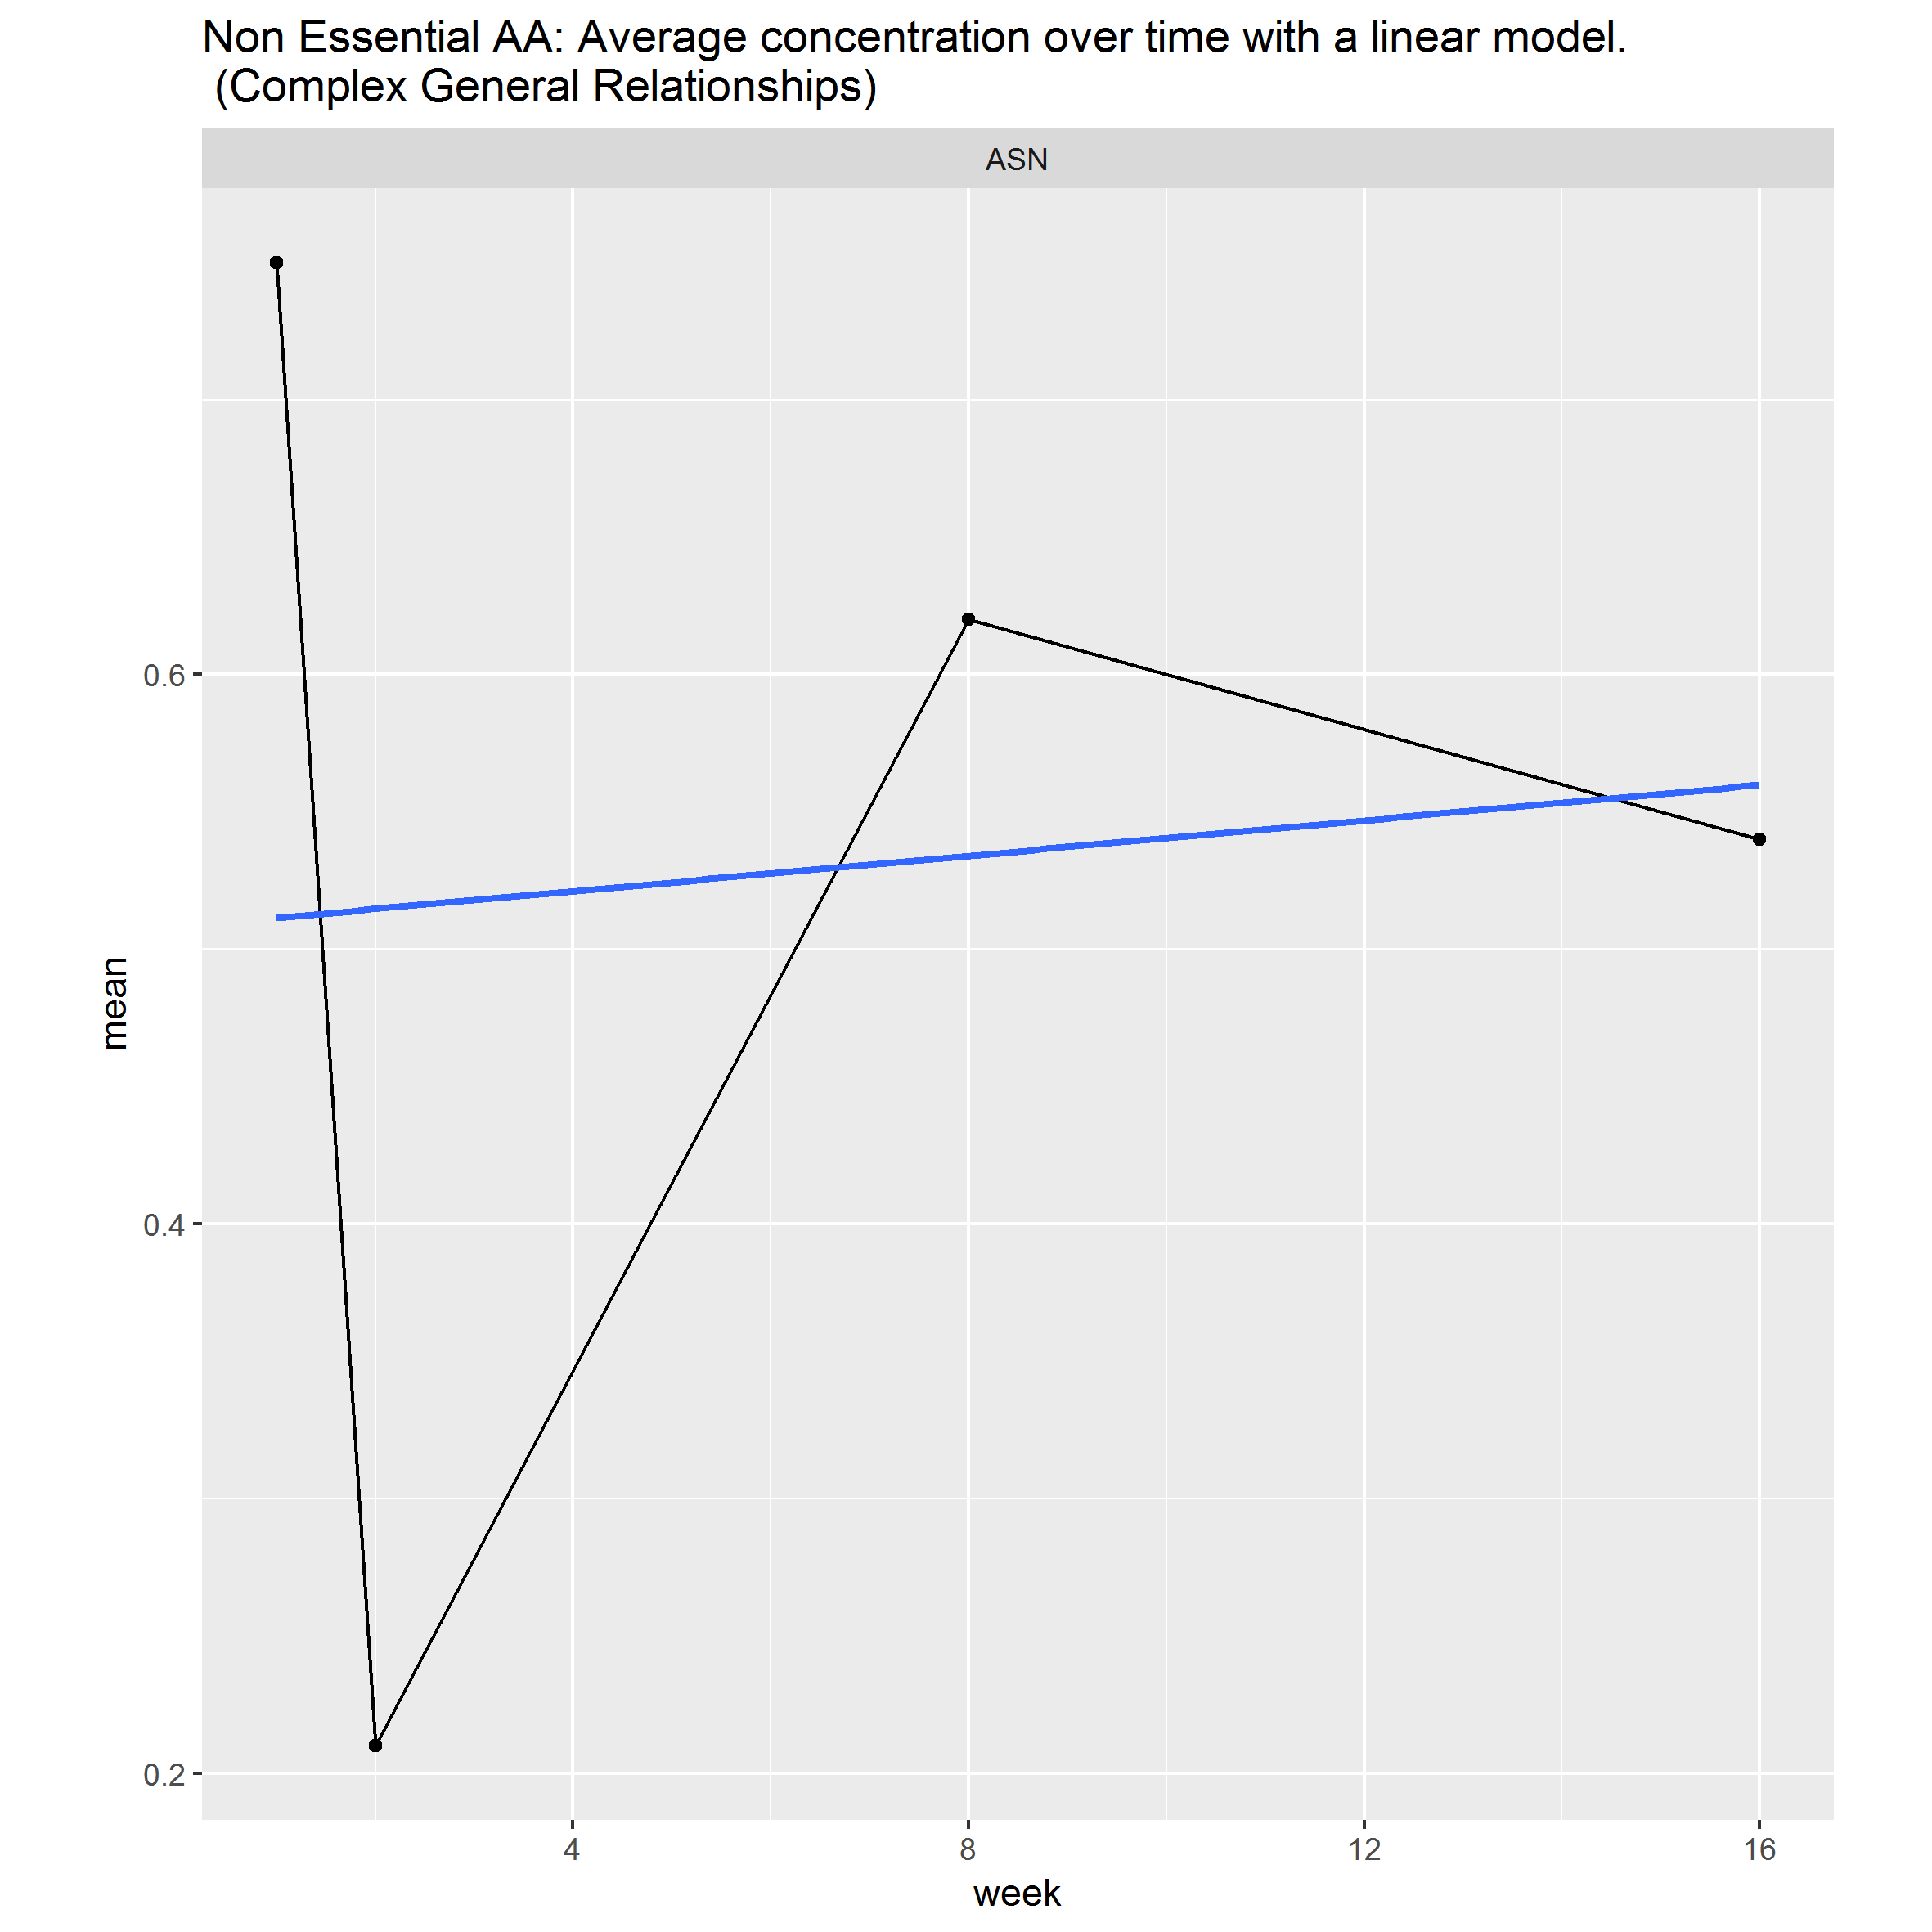
\includegraphics[width= \textwidth]{../week/NEAA_complex.png}
  \caption{Mean concentration per week with a linear regression line in blue. Non essential amino acid ALA has a non significant week effect.}
  \label{fig:NEAA_complex}
\end{figure}


\section{Are AA levels different in the milk for boys and girls?}

There is a time effect for most amino acids. Now I am interested in studying whether the milk for boys and girls has different concentrations. Now the model:

\begin{equation} \label{eq:model2}
  AA = \alpha_0 + \alpha_1 \ week + \alpha_2 \ sex + \alpha_{id}
\end{equation}

has an additional effect that depends on the infant gender - $\alpha_2$. The rest of the coefficients are the same as before. This effect is only present for boys. So another way of writing model \ref{eq:model2} is:

\begin{equation*} \label{eq:model2a}
  AA =  \[ \begin{cases}
  \alpha_0 + \alpha_1 \ week + \alpha_2 + \alpha_{id} & if \  boy, \\
      \alpha_0 + \alpha_1 \ week + \alpha_{id} & if \ girl.
   \end{cases}
\]
\end{equation*}

The coeffient for sex describes the difference in concentration between boys and girls. If $\alpha_2 > 0$, then boys have a higher concentration of that particular amino acid, if it is $0$, there is no difference and when the coeffient is negative, girls have a higher concentration.

\subsection{Essential Amino Acids}

There is no significant differences for all of the essential amino acids. Figure \ref{fig:EAA_coeff} shows the estimated coefficients. Most of the amino acids have a higher concentration for boys except for THR. Once again TRP concentrations are very small and sometimes $0$, so its coeficient is close to $0$ too.

The effects of VAL, HIS, ILE, LEU are similar to those in \cite{NutrientsDutch} and the rest have an oposite sign. In \cite{NutrientsDutch} all of the effects were non significant too.

\begin{figure}[!htb]
  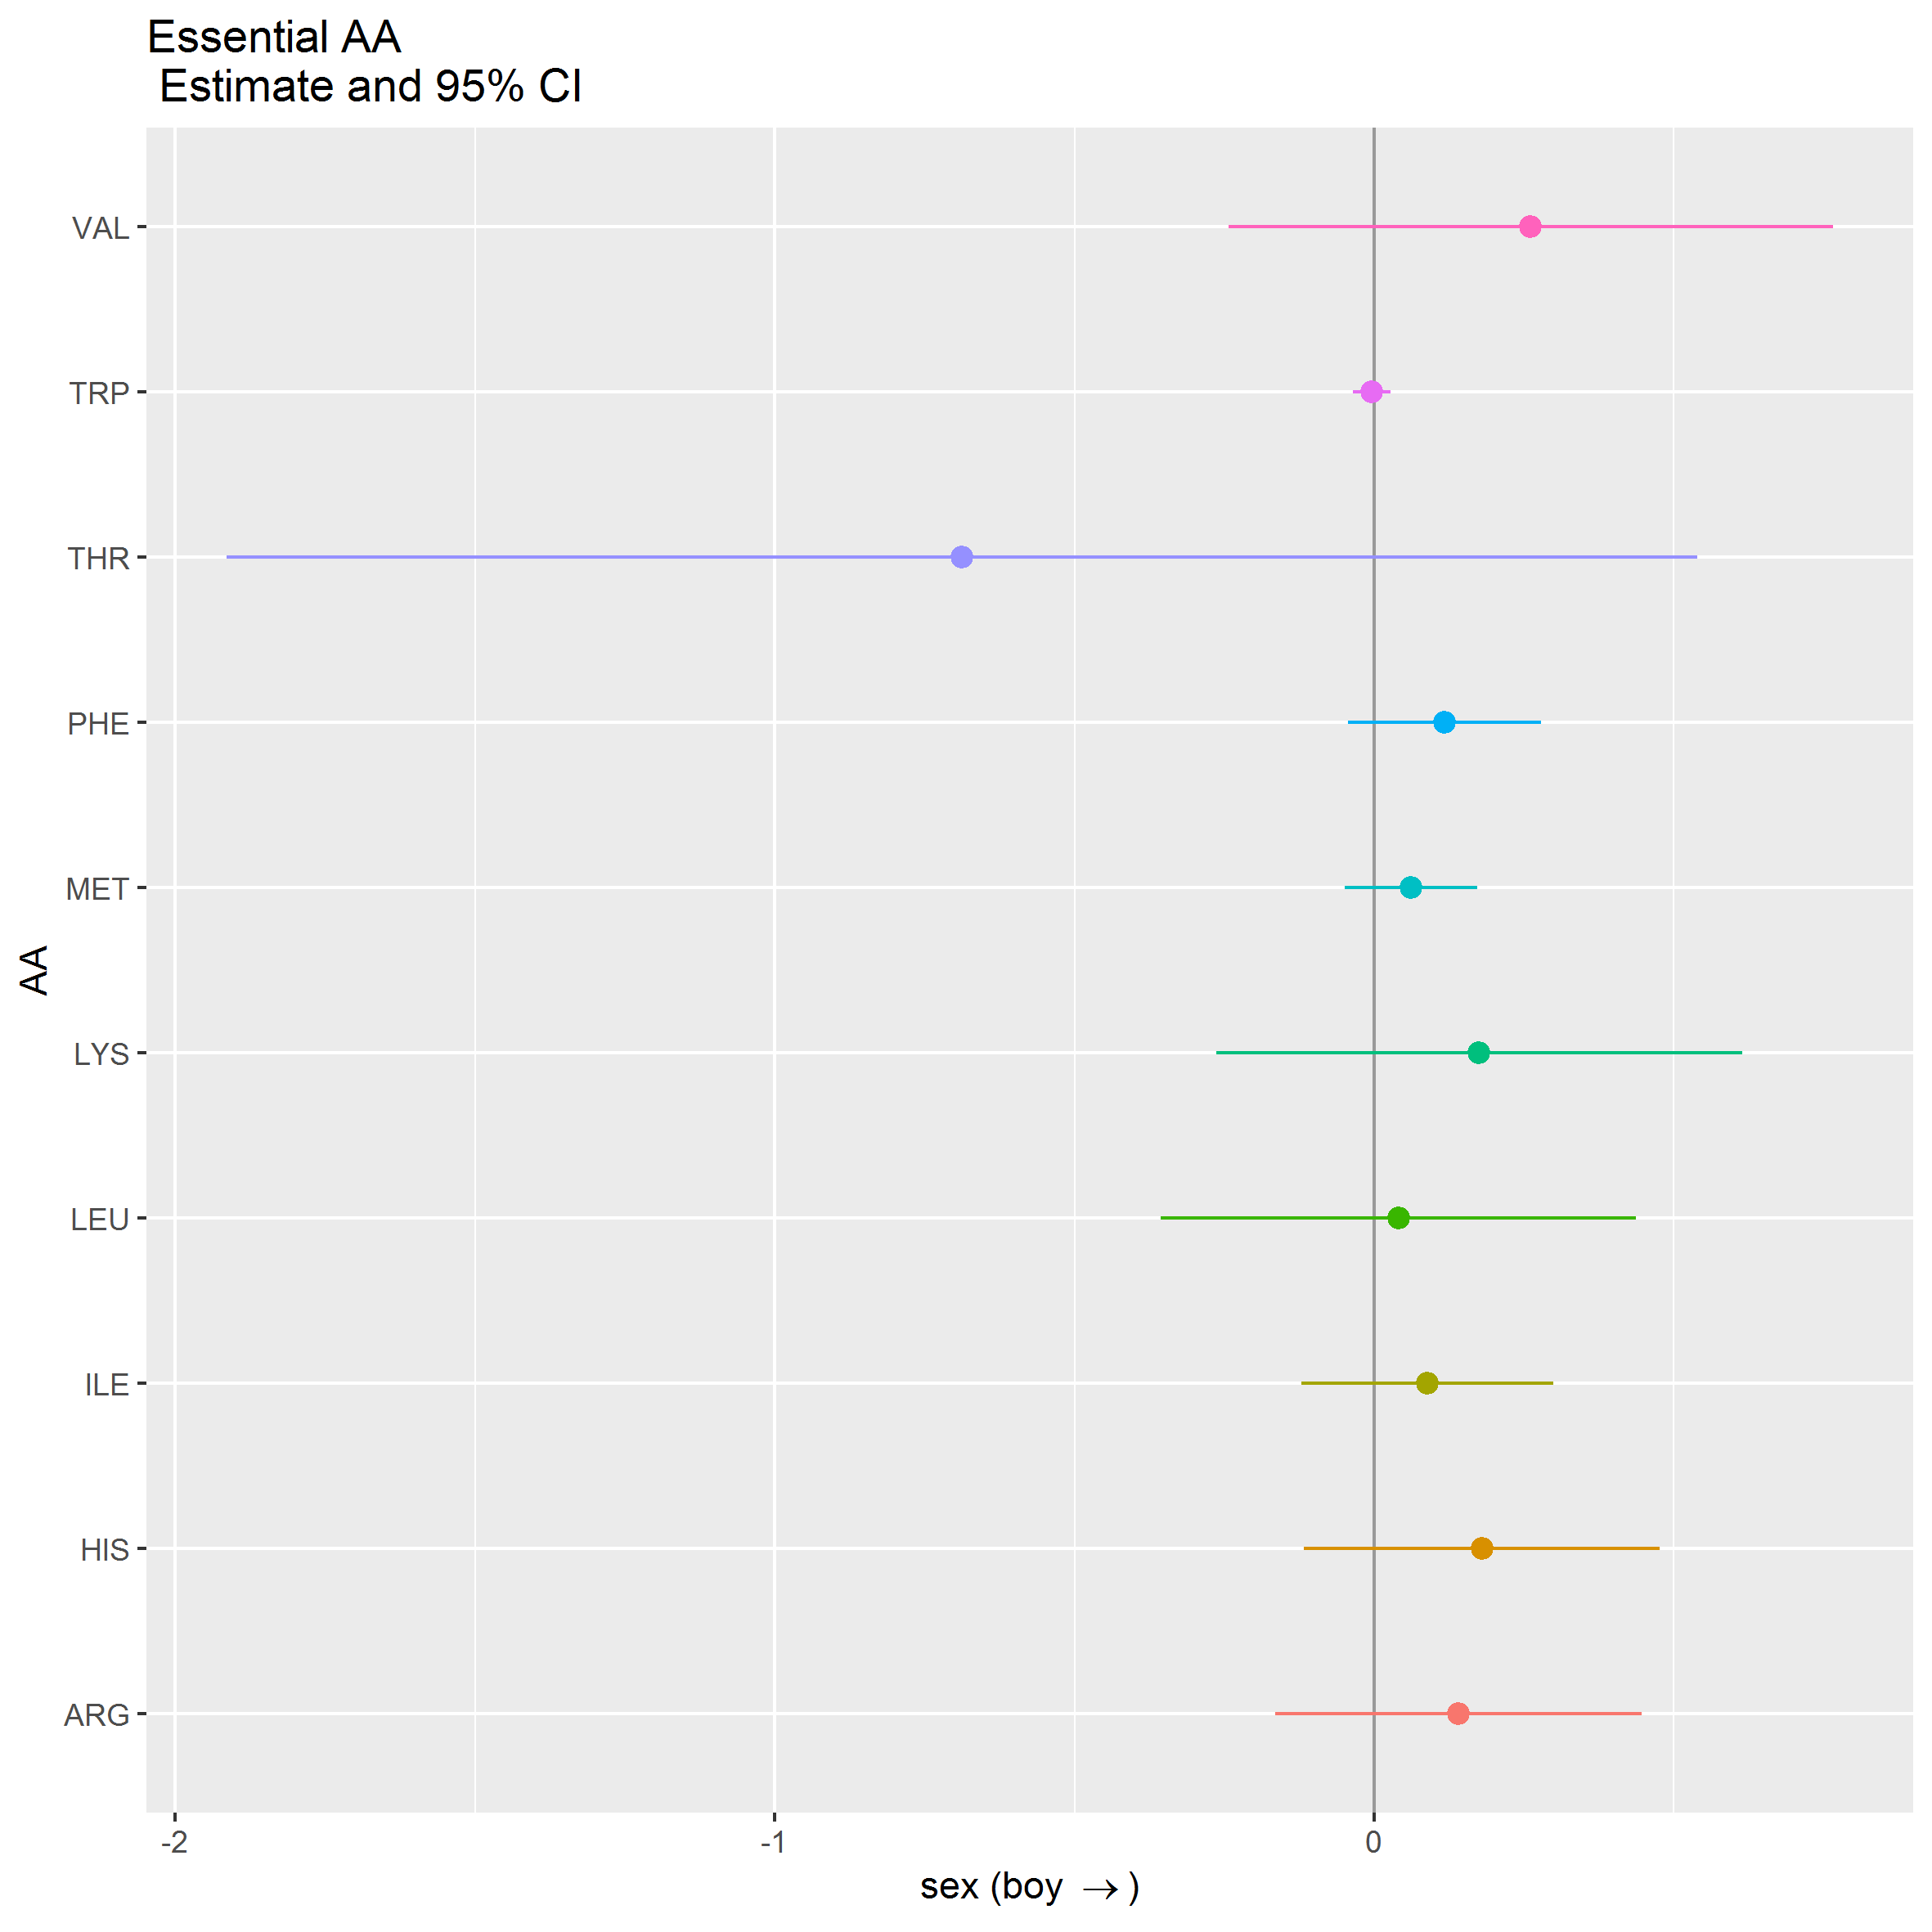
\includegraphics[width= \textwidth]{../sex/EAA_coeff.png}
  \caption{Sex coefficients of model (\ref{eq:model2}) for essential amino acids.}
  \label{fig:EAA_coeff}
\end{figure}


\subsection{Non Essential Amino Acids}

For non essential amino acids some effects are significant and their sign coincide with the estimations found in \cite{NutrientsDutch}.

The effects of GLU, GLN, GLY, ALA, SER, ASP have the same sign as those in \cite{NutrientsDutch}. On the other hand, TYR, ARG, ASN have opposite signs.

In figures \ref{fig:NEAA_coeff} and \ref{fig:NEAA_coeff_detail}, there are $4$ significant differences for girls and boys. They correspond to amino acids GLU, GLY, TYR and CYS. The effects of GLU and GLY have the same sign as in article \cite{NutrientsDutch} but here they are significant.

In the study \cite{NutrientsDutch}, they could not measure CYS. Here it has a significant difference.

Finally, the sign of TYR is different from that in \cite{NutrientsDutch} but here it has a signinficant effect.

\begin{figure}[!htb]
  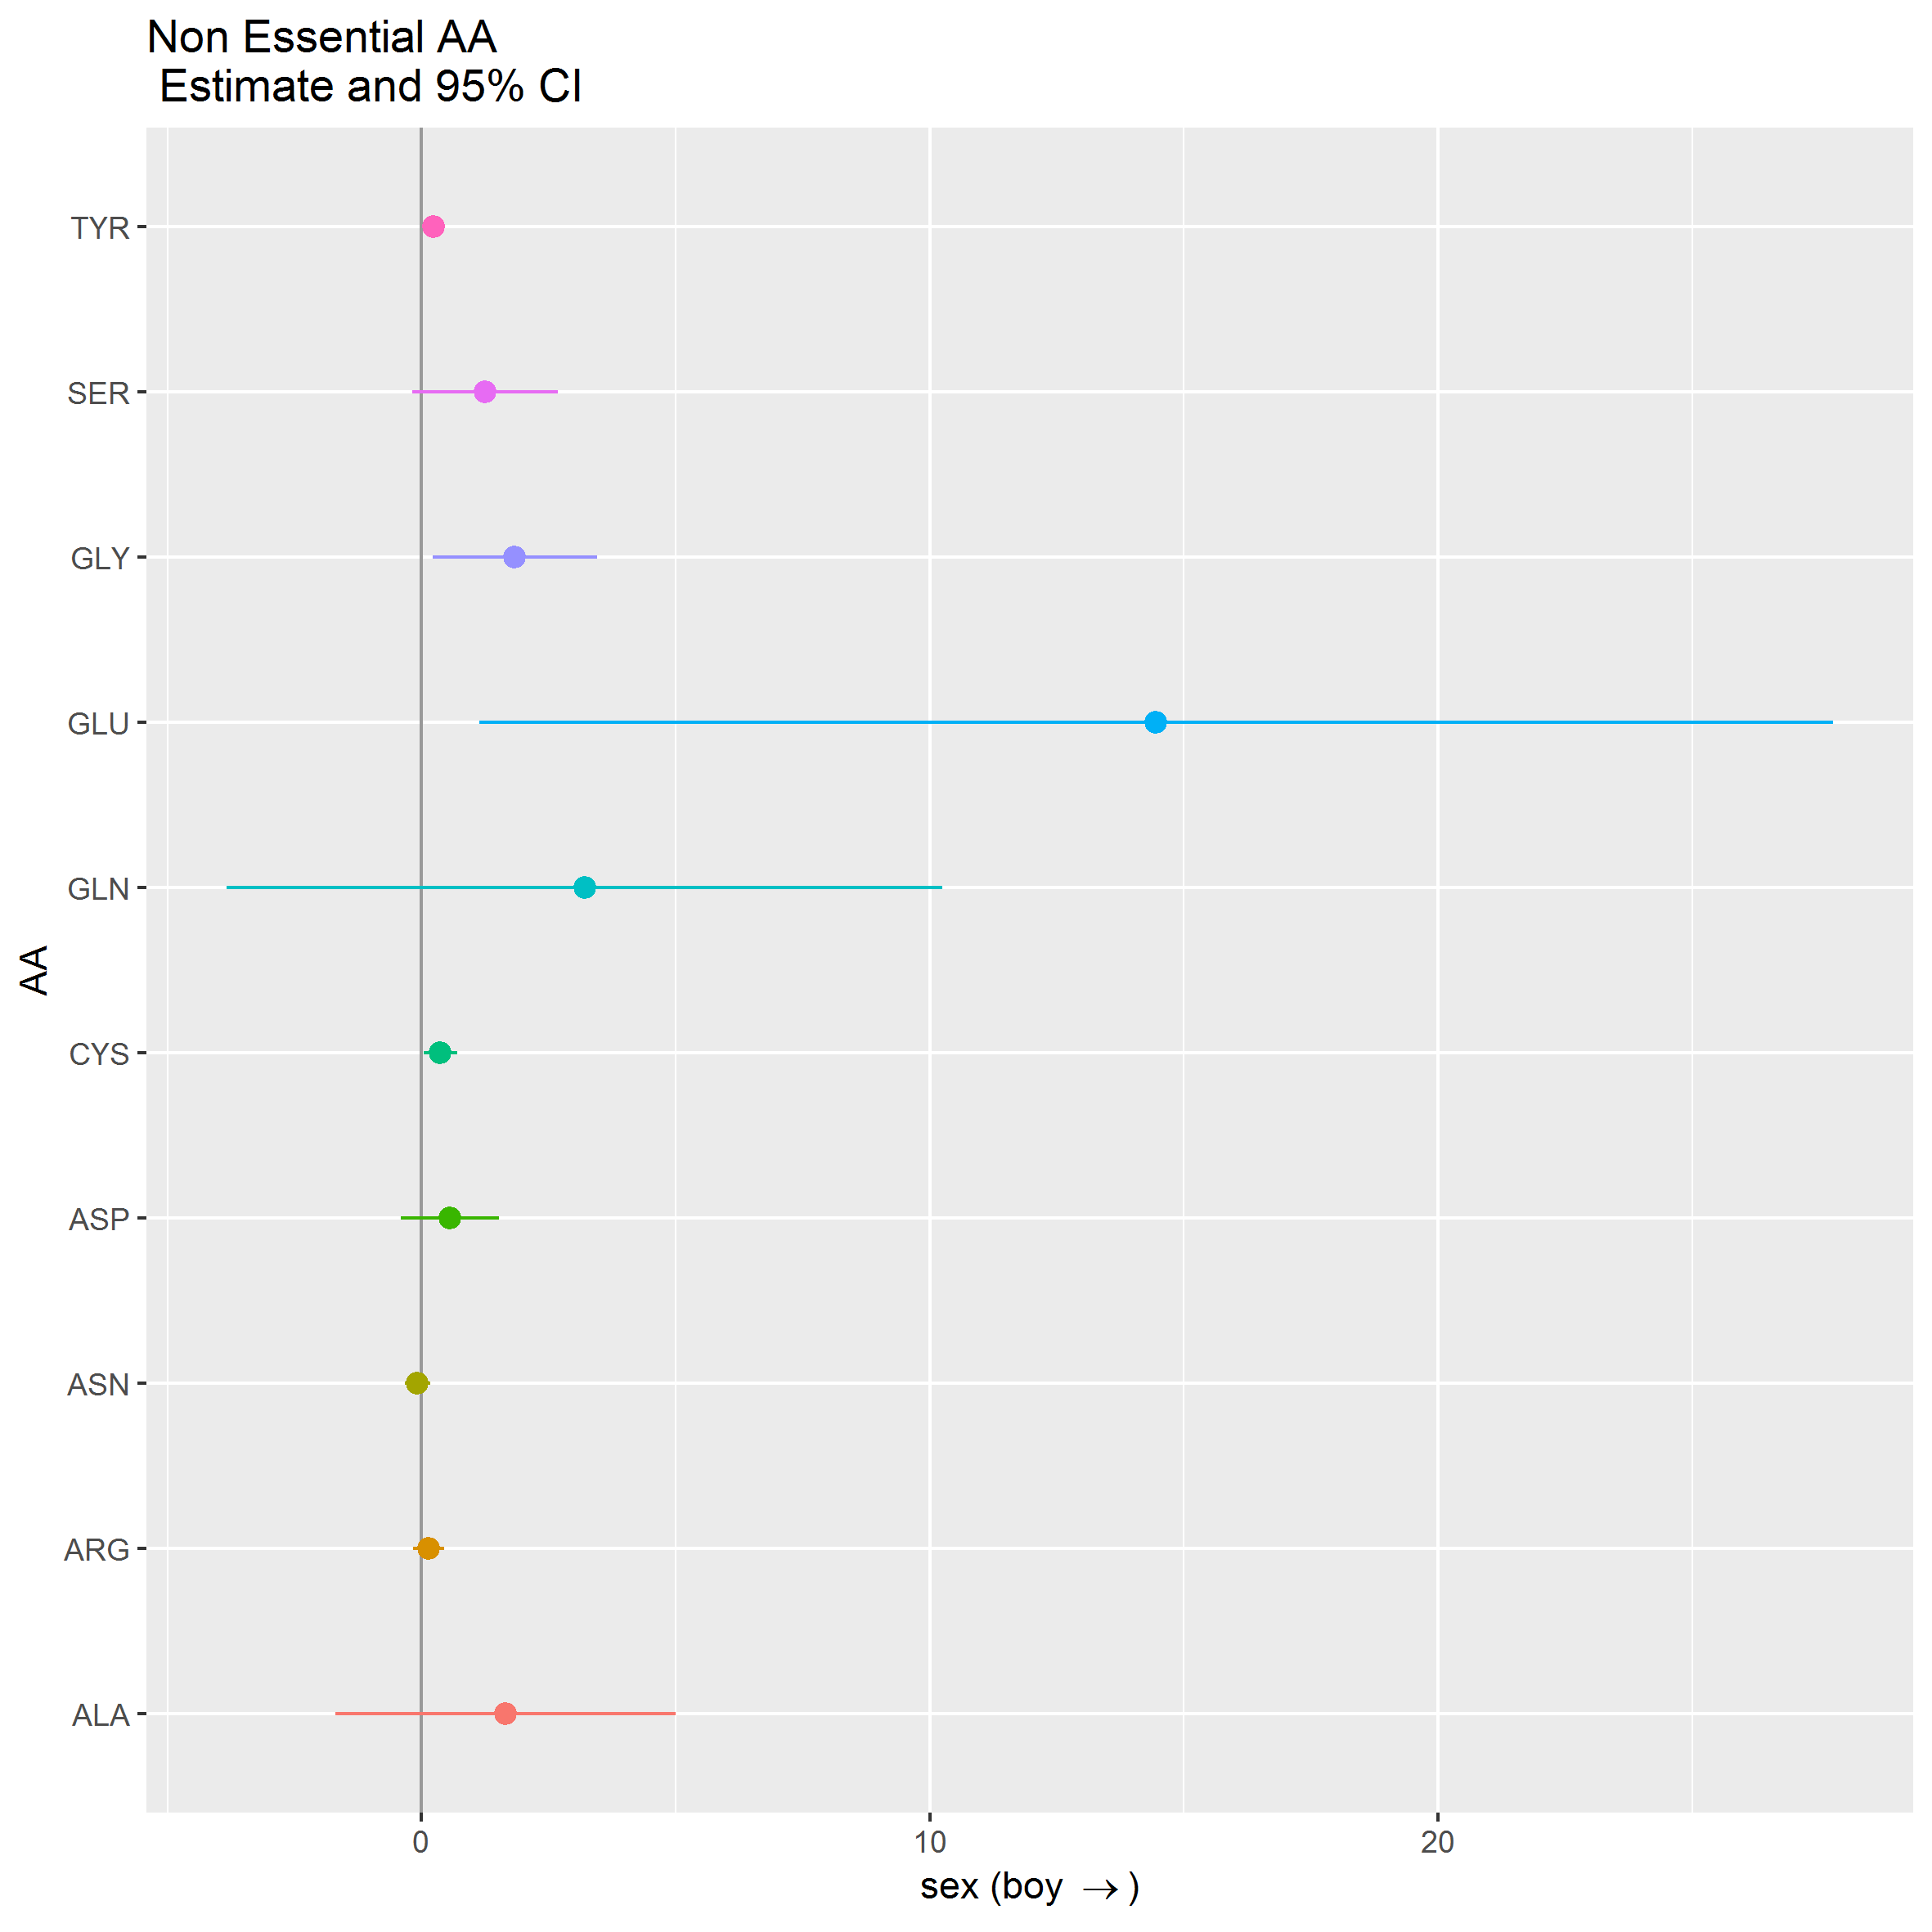
\includegraphics[width= \textwidth]{../sex/NEAA_coeff.png}
  \caption{Sex coefficients of model (\ref{eq:model2}) for non essential amino acids.}
  \label{fig:NEAA_coeff}
\end{figure}

\begin{figure}[!htb]
  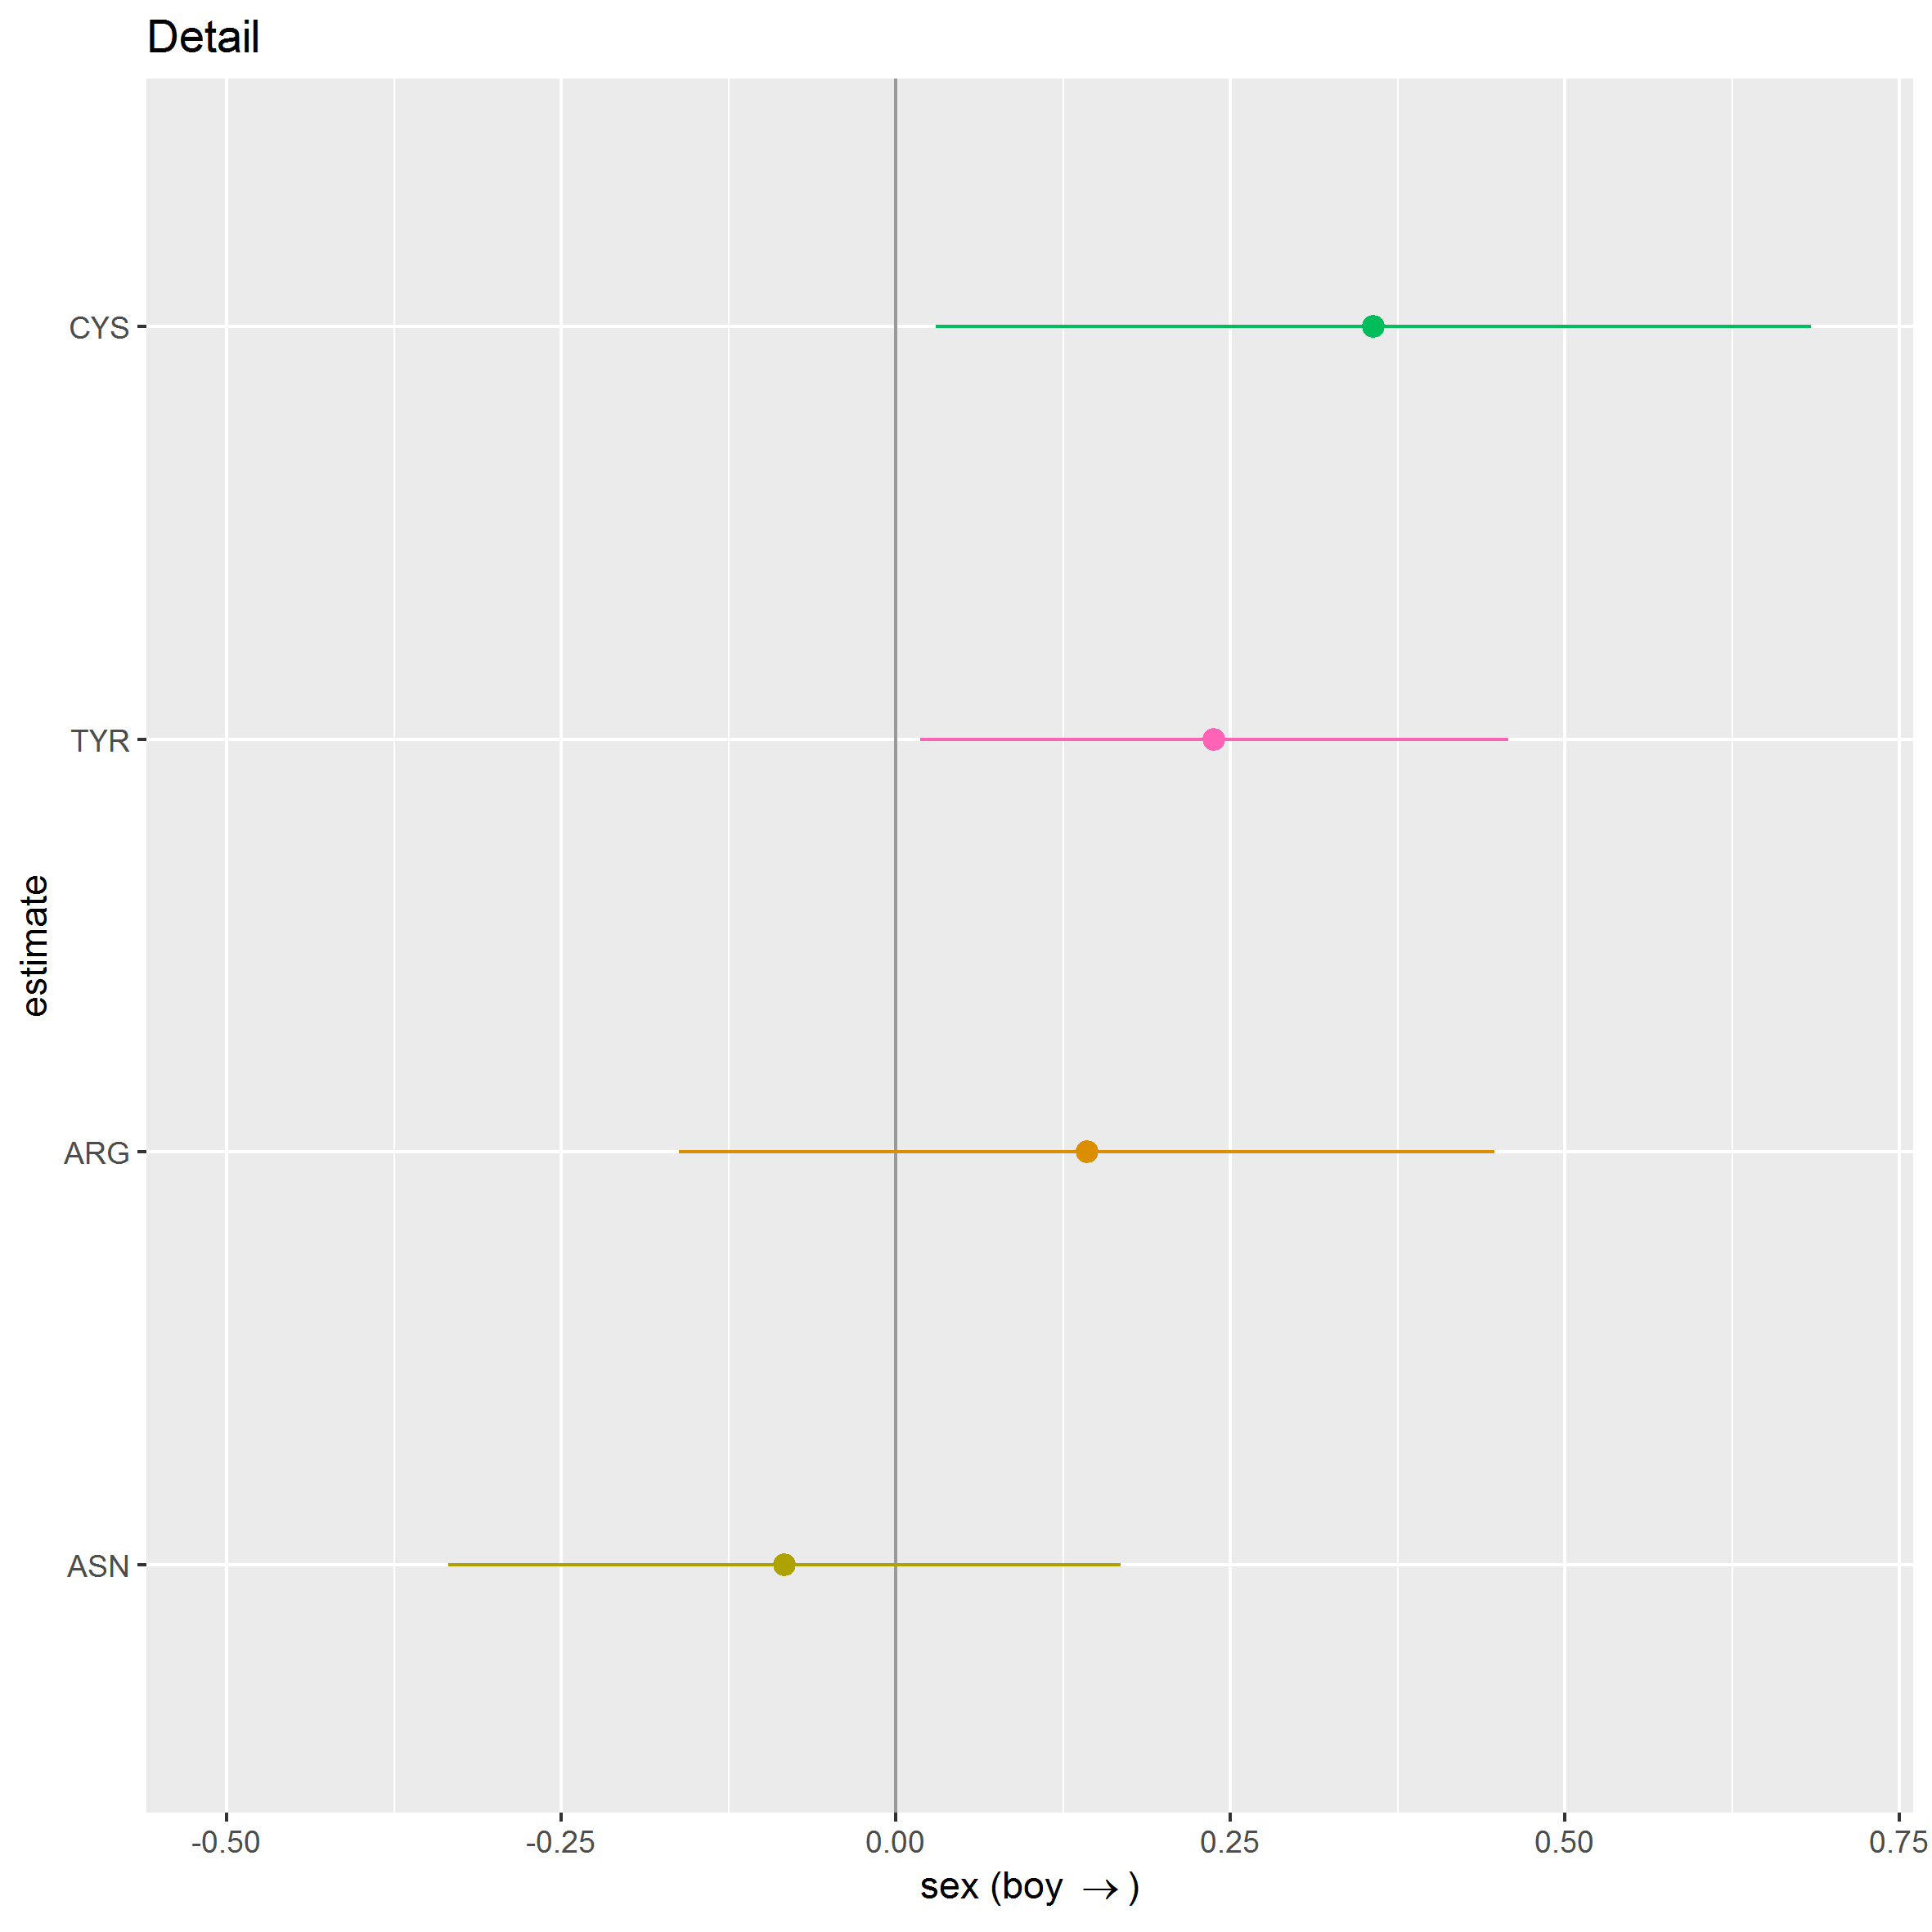
\includegraphics[width= \textwidth]{../sex/NEAA_coeff_detail.png}
  \caption{Detail of the sex coefficients of model (\ref{eq:model2}) for the non essential amino acids with small effects.}
  \label{fig:NEAA_coeff_detail}
\end{figure}

\begin{figure}[!htb]
  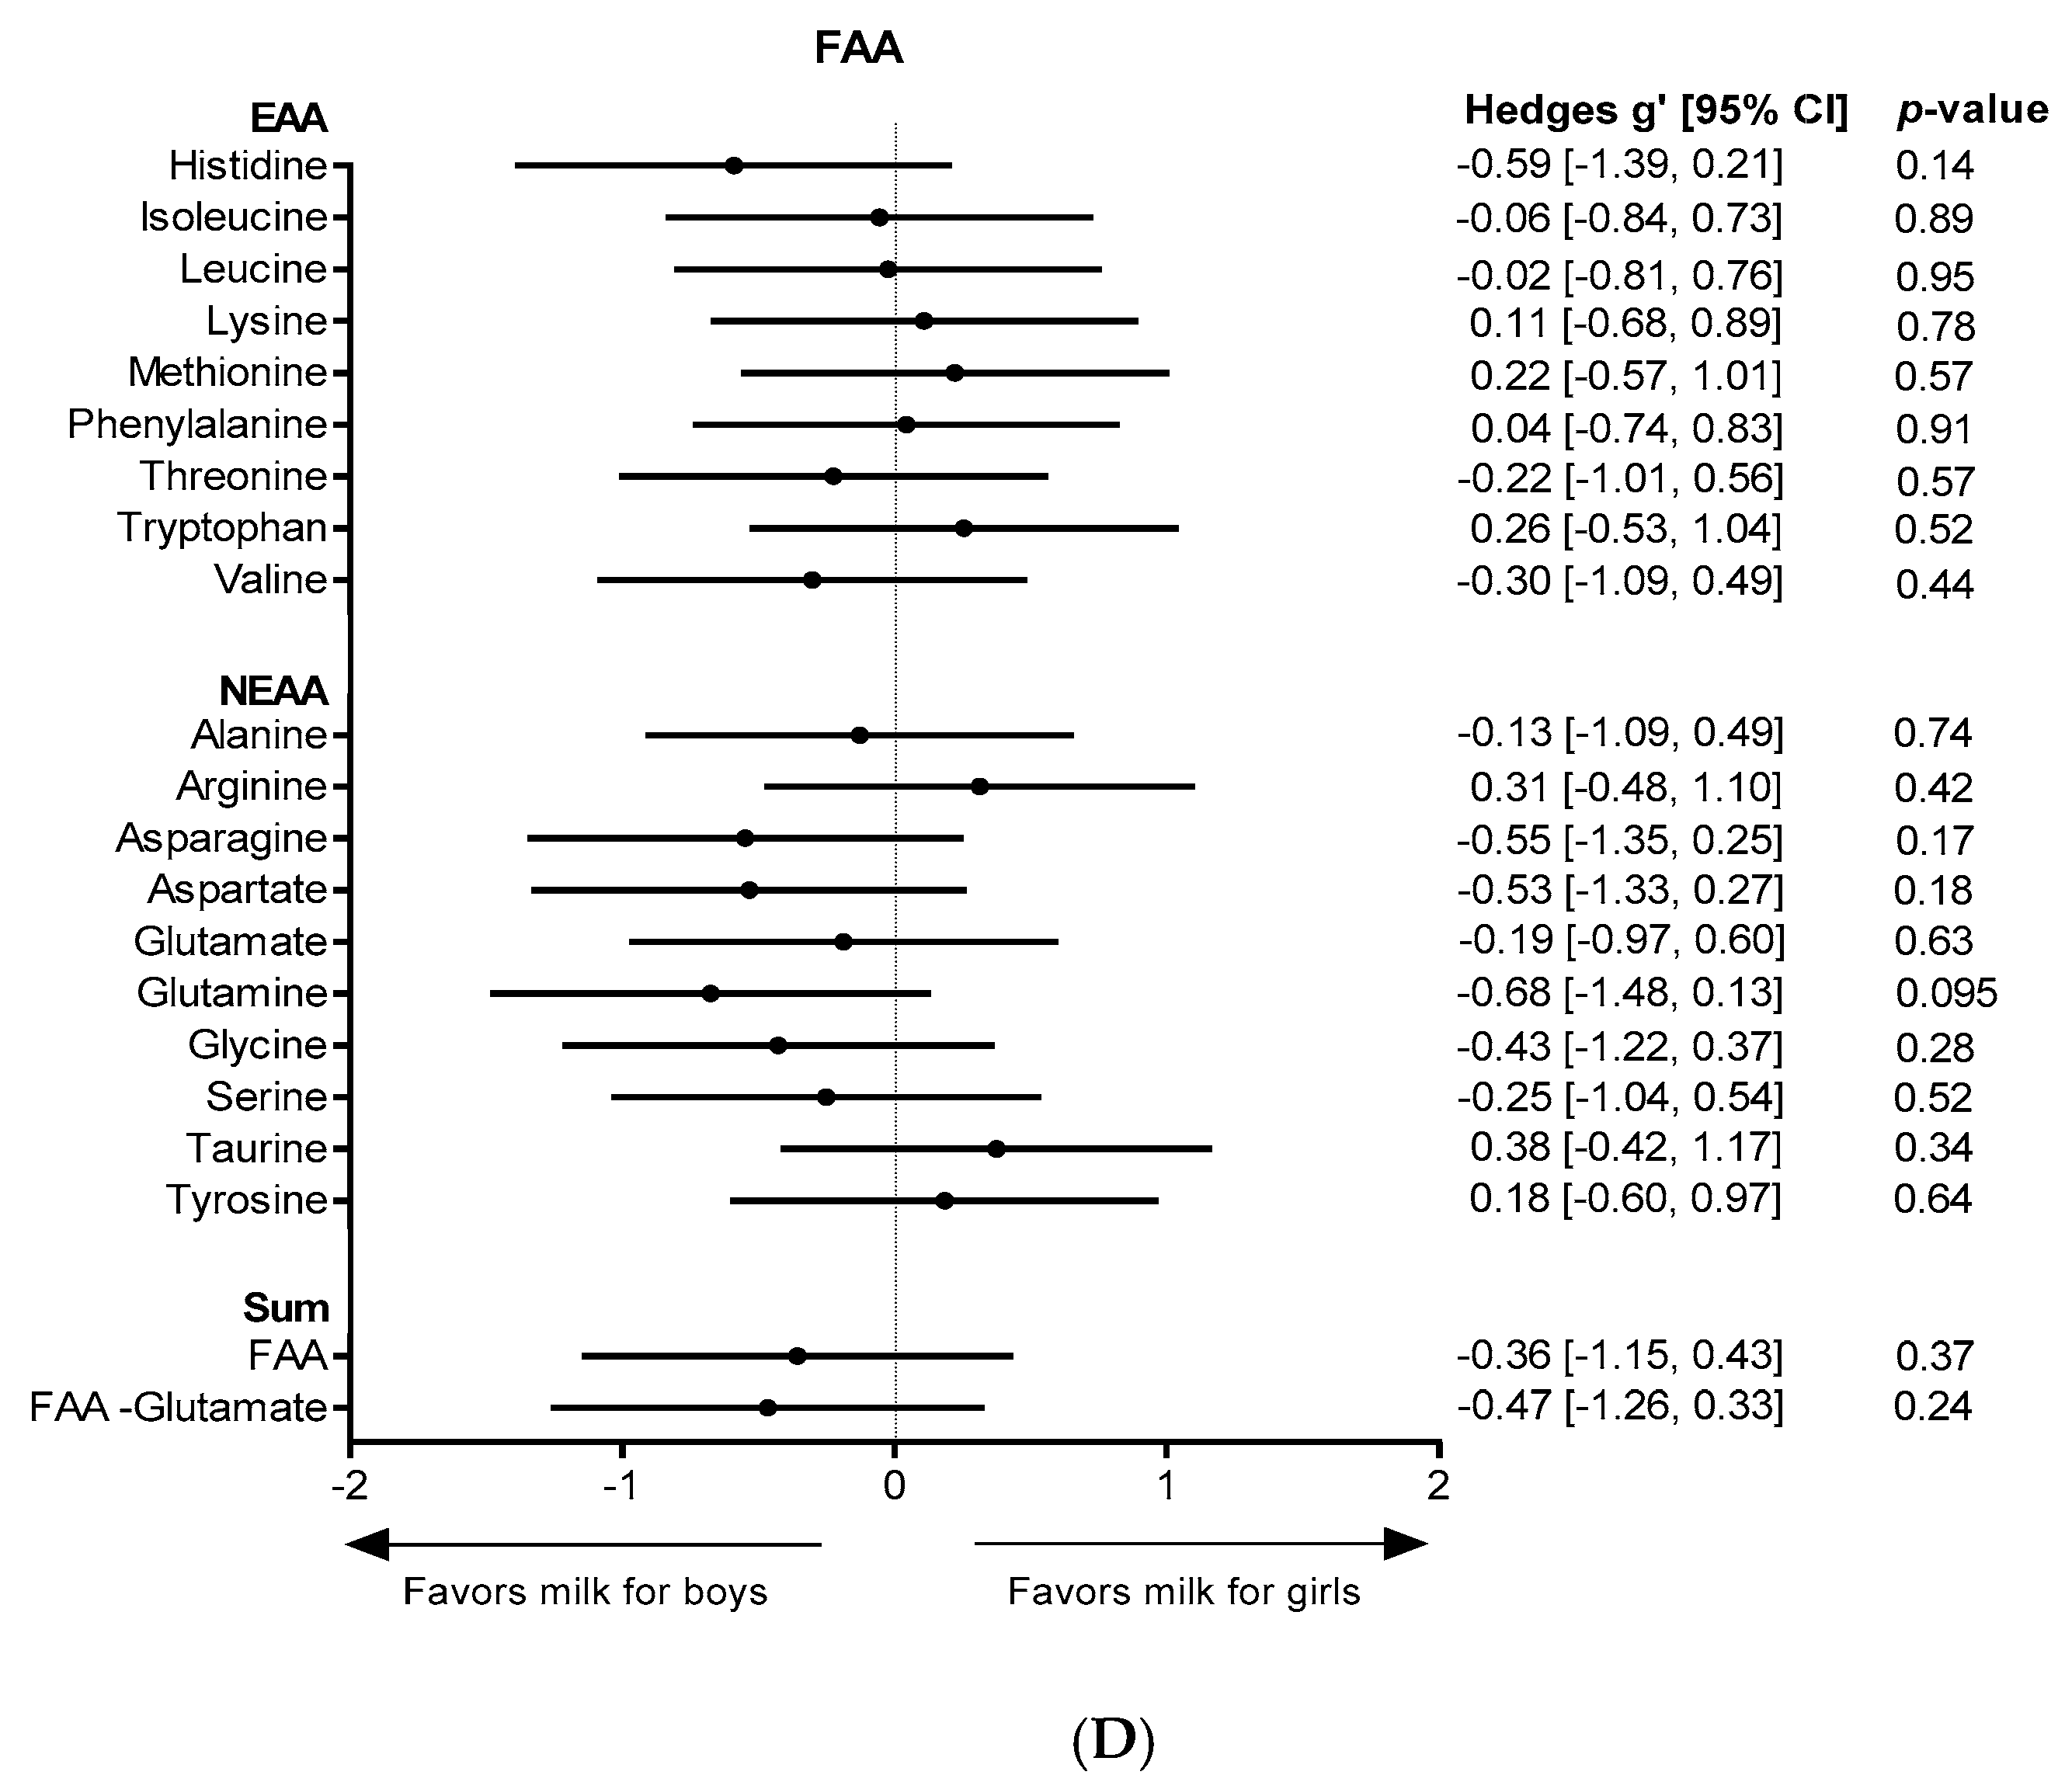
\includegraphics[width= \textwidth]{../sex/nutrientsFAA.png}
  \caption{Sex coefficients found in article \cite{NutrientsDutch}.}
  \label{fig:nutrientsFAA}
\end{figure}

\section{If the concentration changes over time, is it different for boys and girls?}

Now we know that there is a time effect for almost all amino acids and a sex effect for $4$ non essential amino acids (GLU, GLY, TYR and CYS). The question now is whether the variation of concentration over time changes for girls and boys.

For the model I add yet another effect:

\begin{equation} \label{eq:model3}
  AA = \alpha_0 + \alpha_1 \ week + \alpha_2 \ sex + \alpha_3 \ week \times sex + \alpha_{id}
\end{equation}

where the coeffient $\alpha_3$, that corresponds to the interaction term $week \times sex$, can be interpreted in two different ways. First by rewriting model \ref{eq:model3} as:

\begin{equation} \label{eq:model3a}
  AA = \alpha_0 + \left(\alpha_1  + \alpha_3 \ sex \right) \times \ week + \alpha_2 \ sex  + \alpha_{id}
\end{equation}

you can read $\alpha_1  + \alpha_3 $ as the time effect for boys and $\alpha_1$ as the time effect for girls. With this notation $\alpha_3$ is the time difference between boys and girls.

The second interpretation follows from the other possible arrangement, namely:

\begin{equation} \label{eq:model3b}
  AA = \alpha_0 + \alpha_1 \ week + \left(\alpha_2  + \alpha_3 \ week \right) \times \ sex  + \alpha_{id}
\end{equation}

here $\alpha_2 + \alpha_3$ is the sex effect per week. So for a given week, the difference between boys and girls is $\alpha_2 + \alpha_3$. As before this difference can be positive, negative or zero.

Either way the interaction coeffient $\alpha_3$ represents a difference over time. So I will focus on this coefficient first.

\subsection{Essential Amino Acids}

As expected, all of these effects are smaller than the main effects. Also the coeffient are non significant. However, the trends suggest that the concentration increases faster for girls over time for all amino acids except HIS. The variation in concentration of essential amino acids over time is similar for boys and girls.

Figure \ref{fig:EAA_girls} shows the amino acids whose concentration increases more repidly over time for girls. For HIS they concentration for boys is bigger over time except at week $8$.

Finally, figure \ref{fig:EAA_TRP} shows TRP. As before it jumps between positive values and $0$.

\begin{figure}[H]
  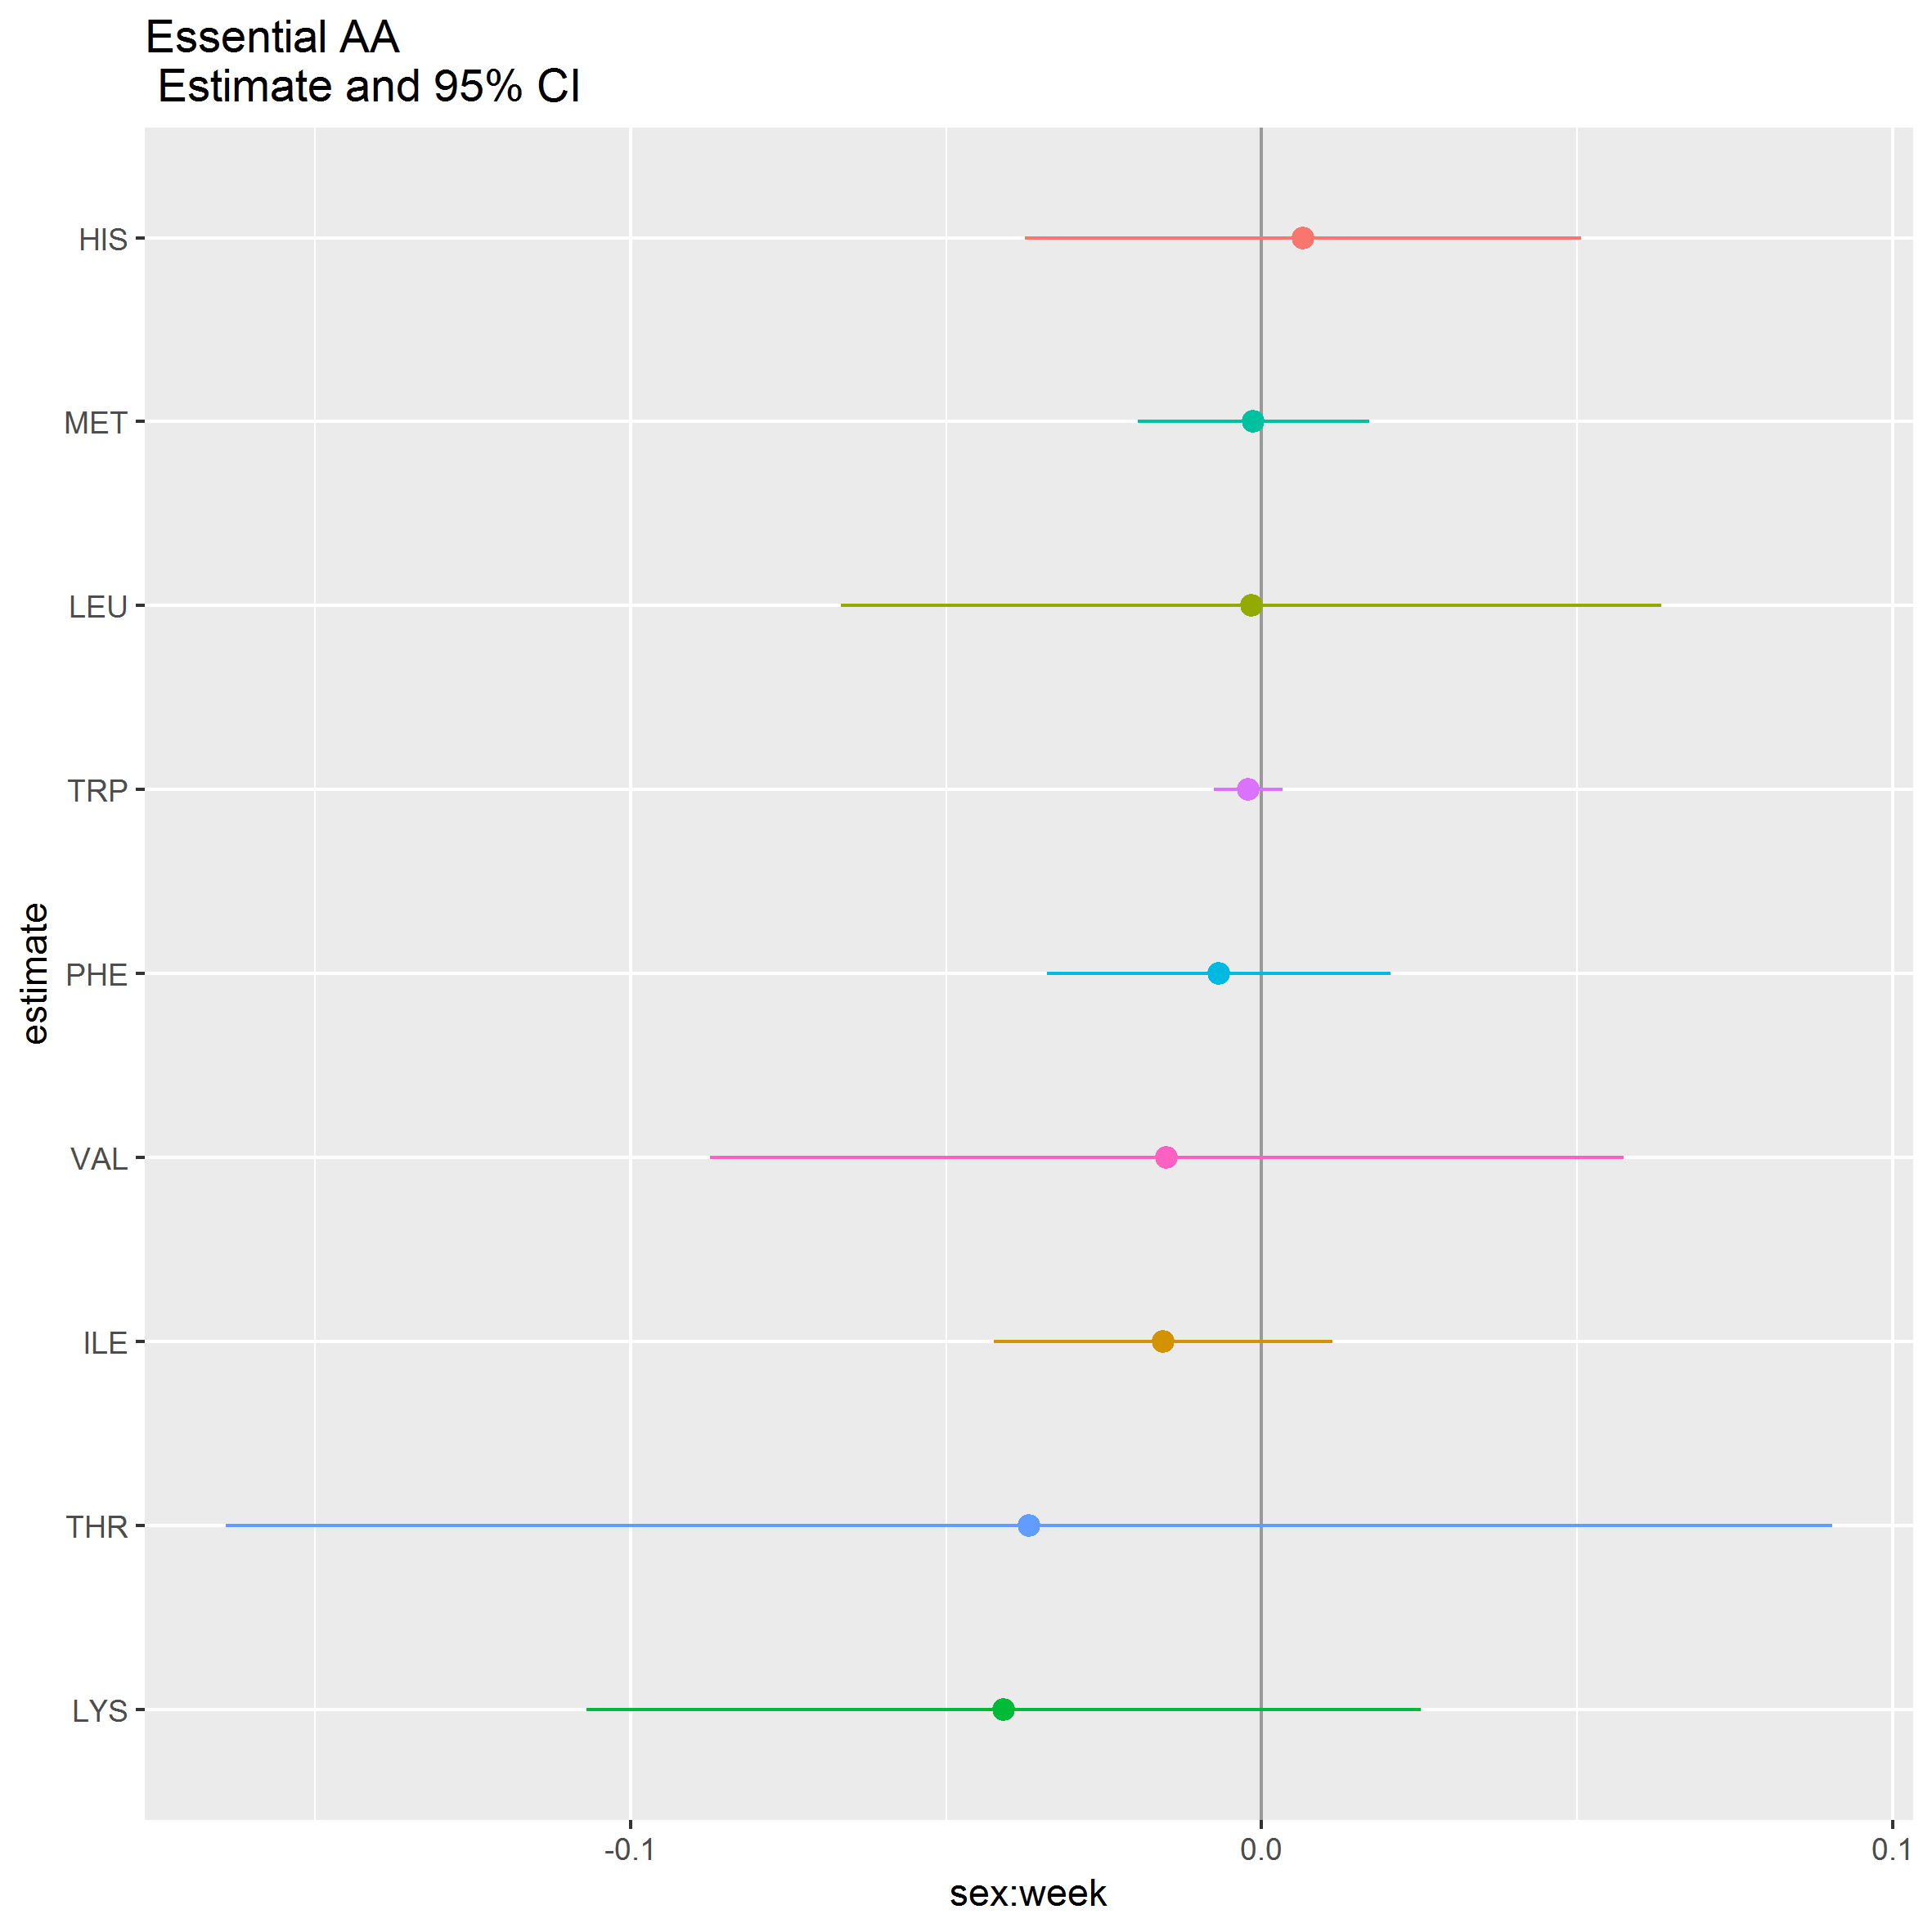
\includegraphics[width= \textwidth]{../sexweek/EAA_SW_SW_coeff.png}
  \caption{$Sex \times week$ coefficients of model (\ref{eq:model3}) for essential amino acids.}
  \label{fig:EAA_SW_SW_coeff}
\end{figure}


\begin{figure}[H]
  \centering
  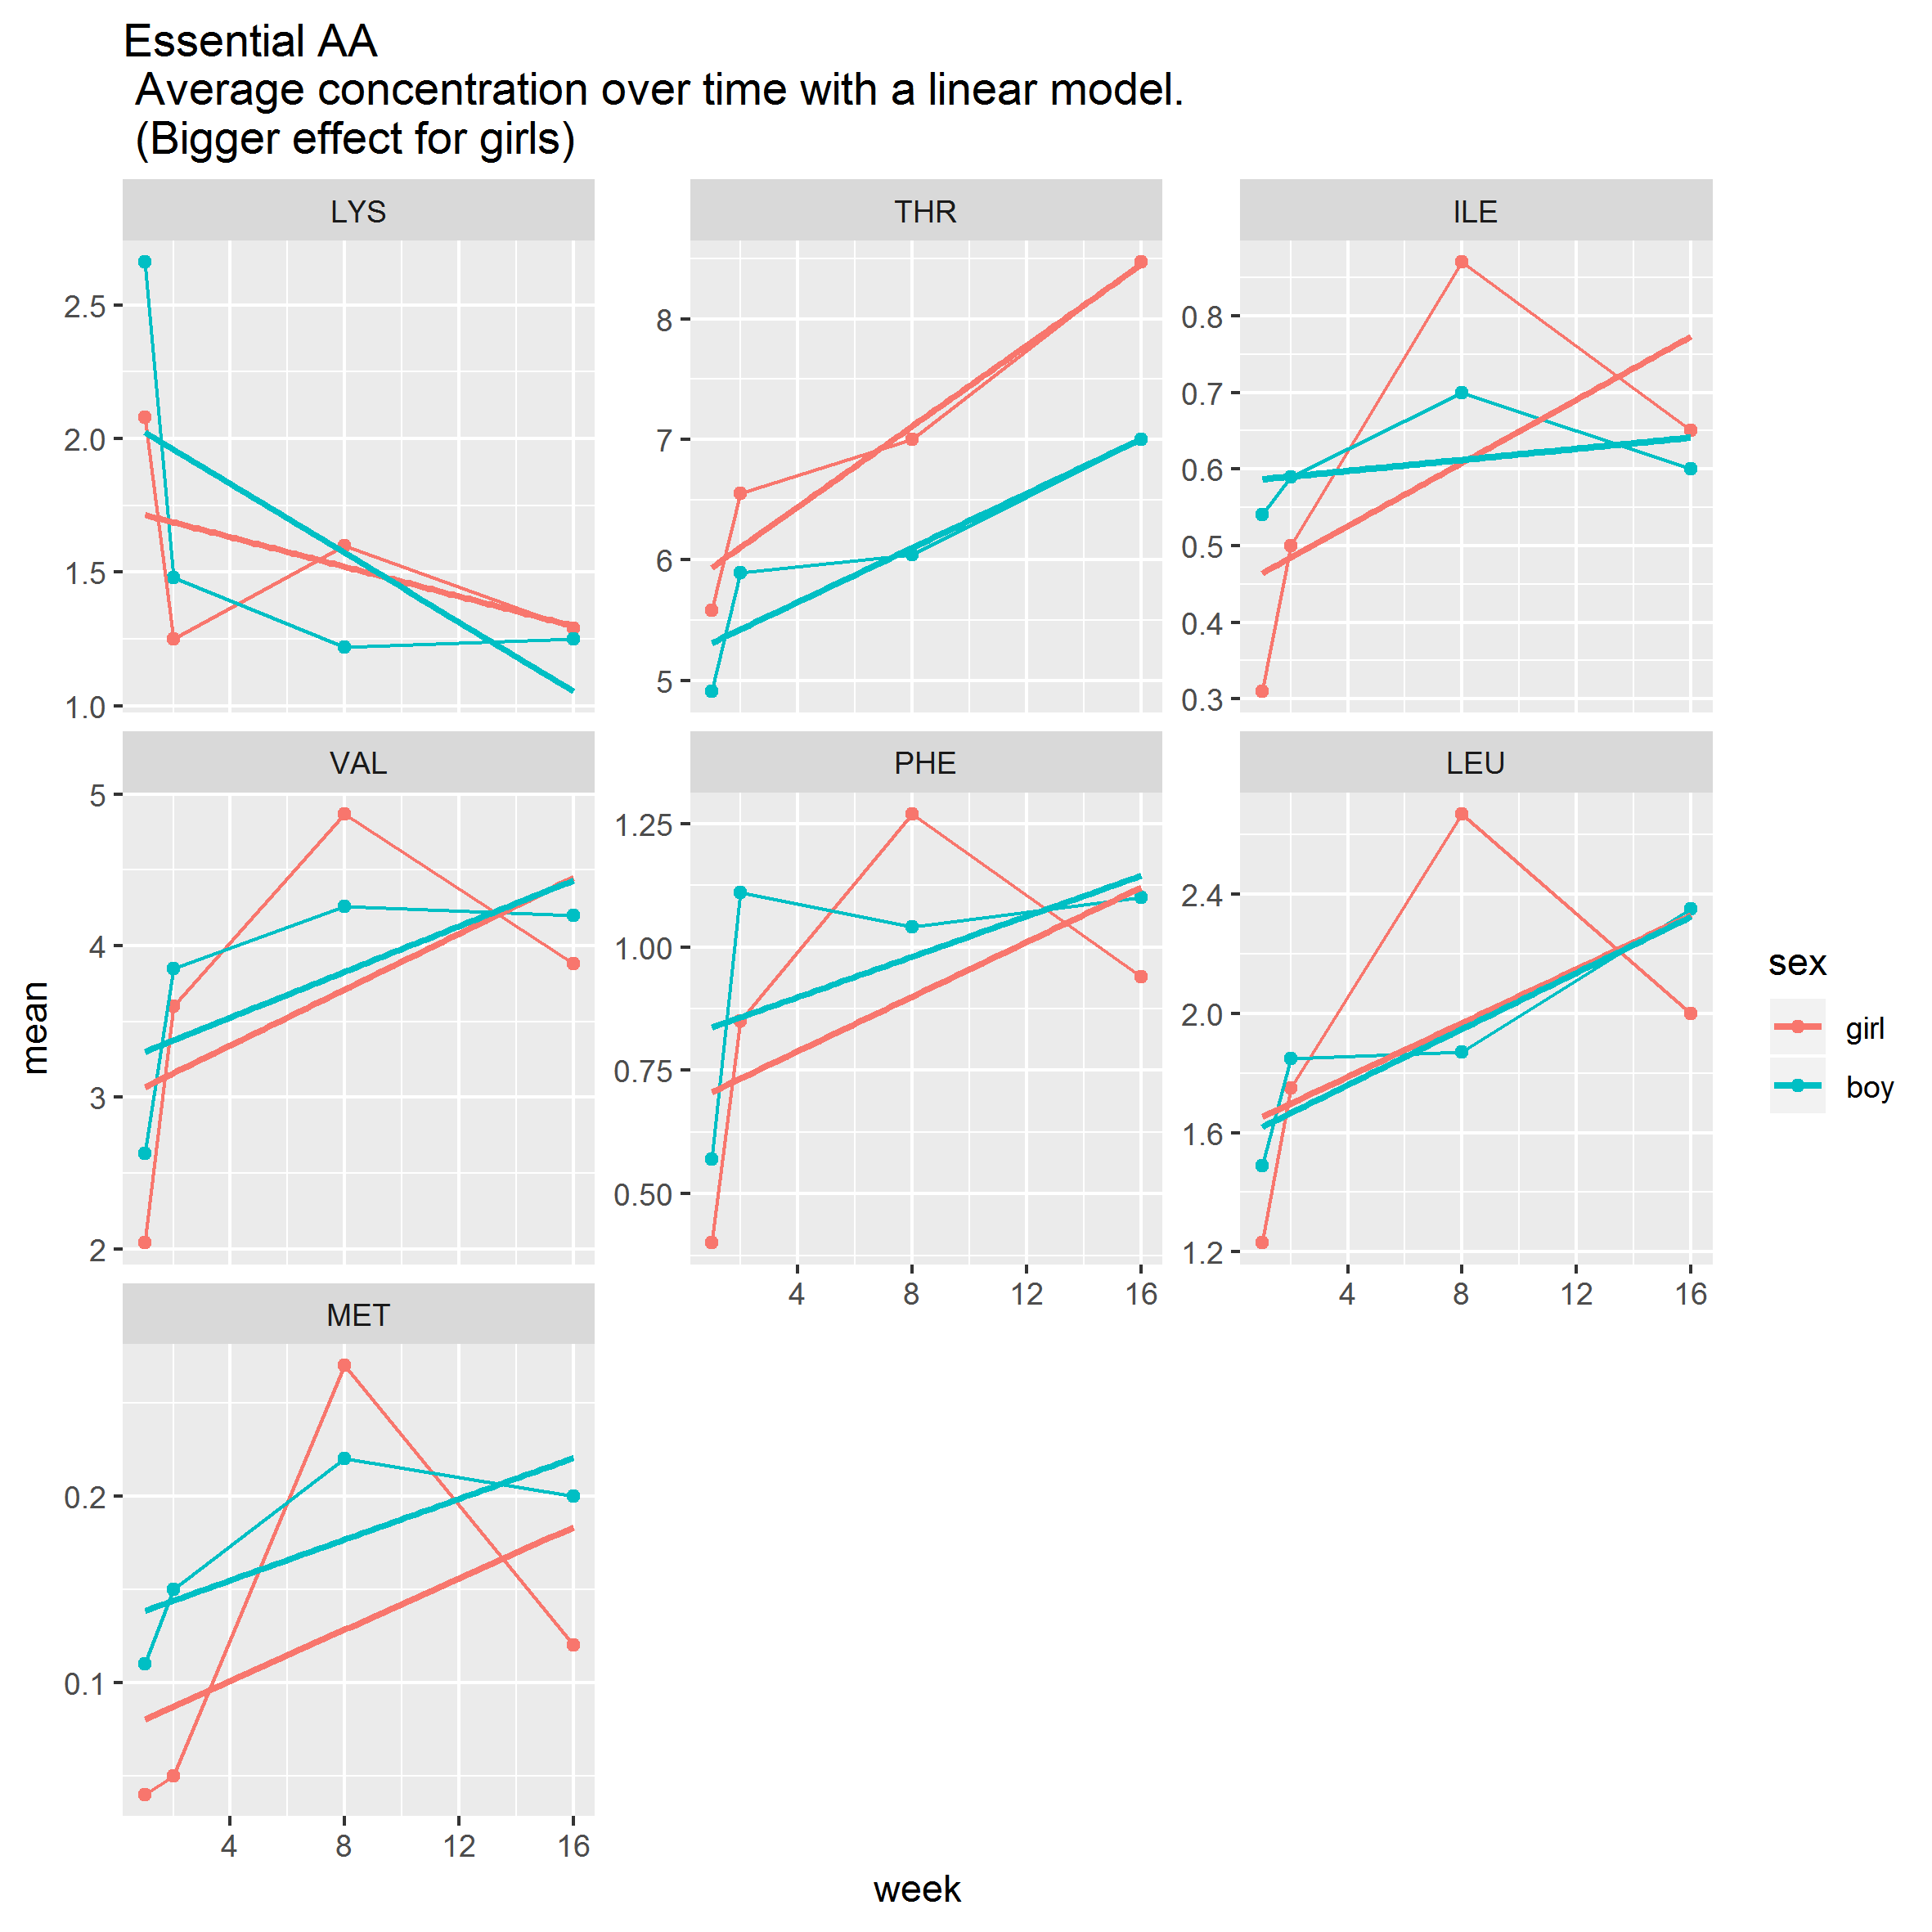
\includegraphics[width=\textwidth]{../sexweek/EAA_girls.png}
  \caption{Mean concentration per week with a linear regression line in blue for boys and pink for girls. Essential amino acids with a bigger interaction effect for girls.}
  \label{fig:EAA_girls}
\end{figure}

\begin{figure}[H]
  \centering
  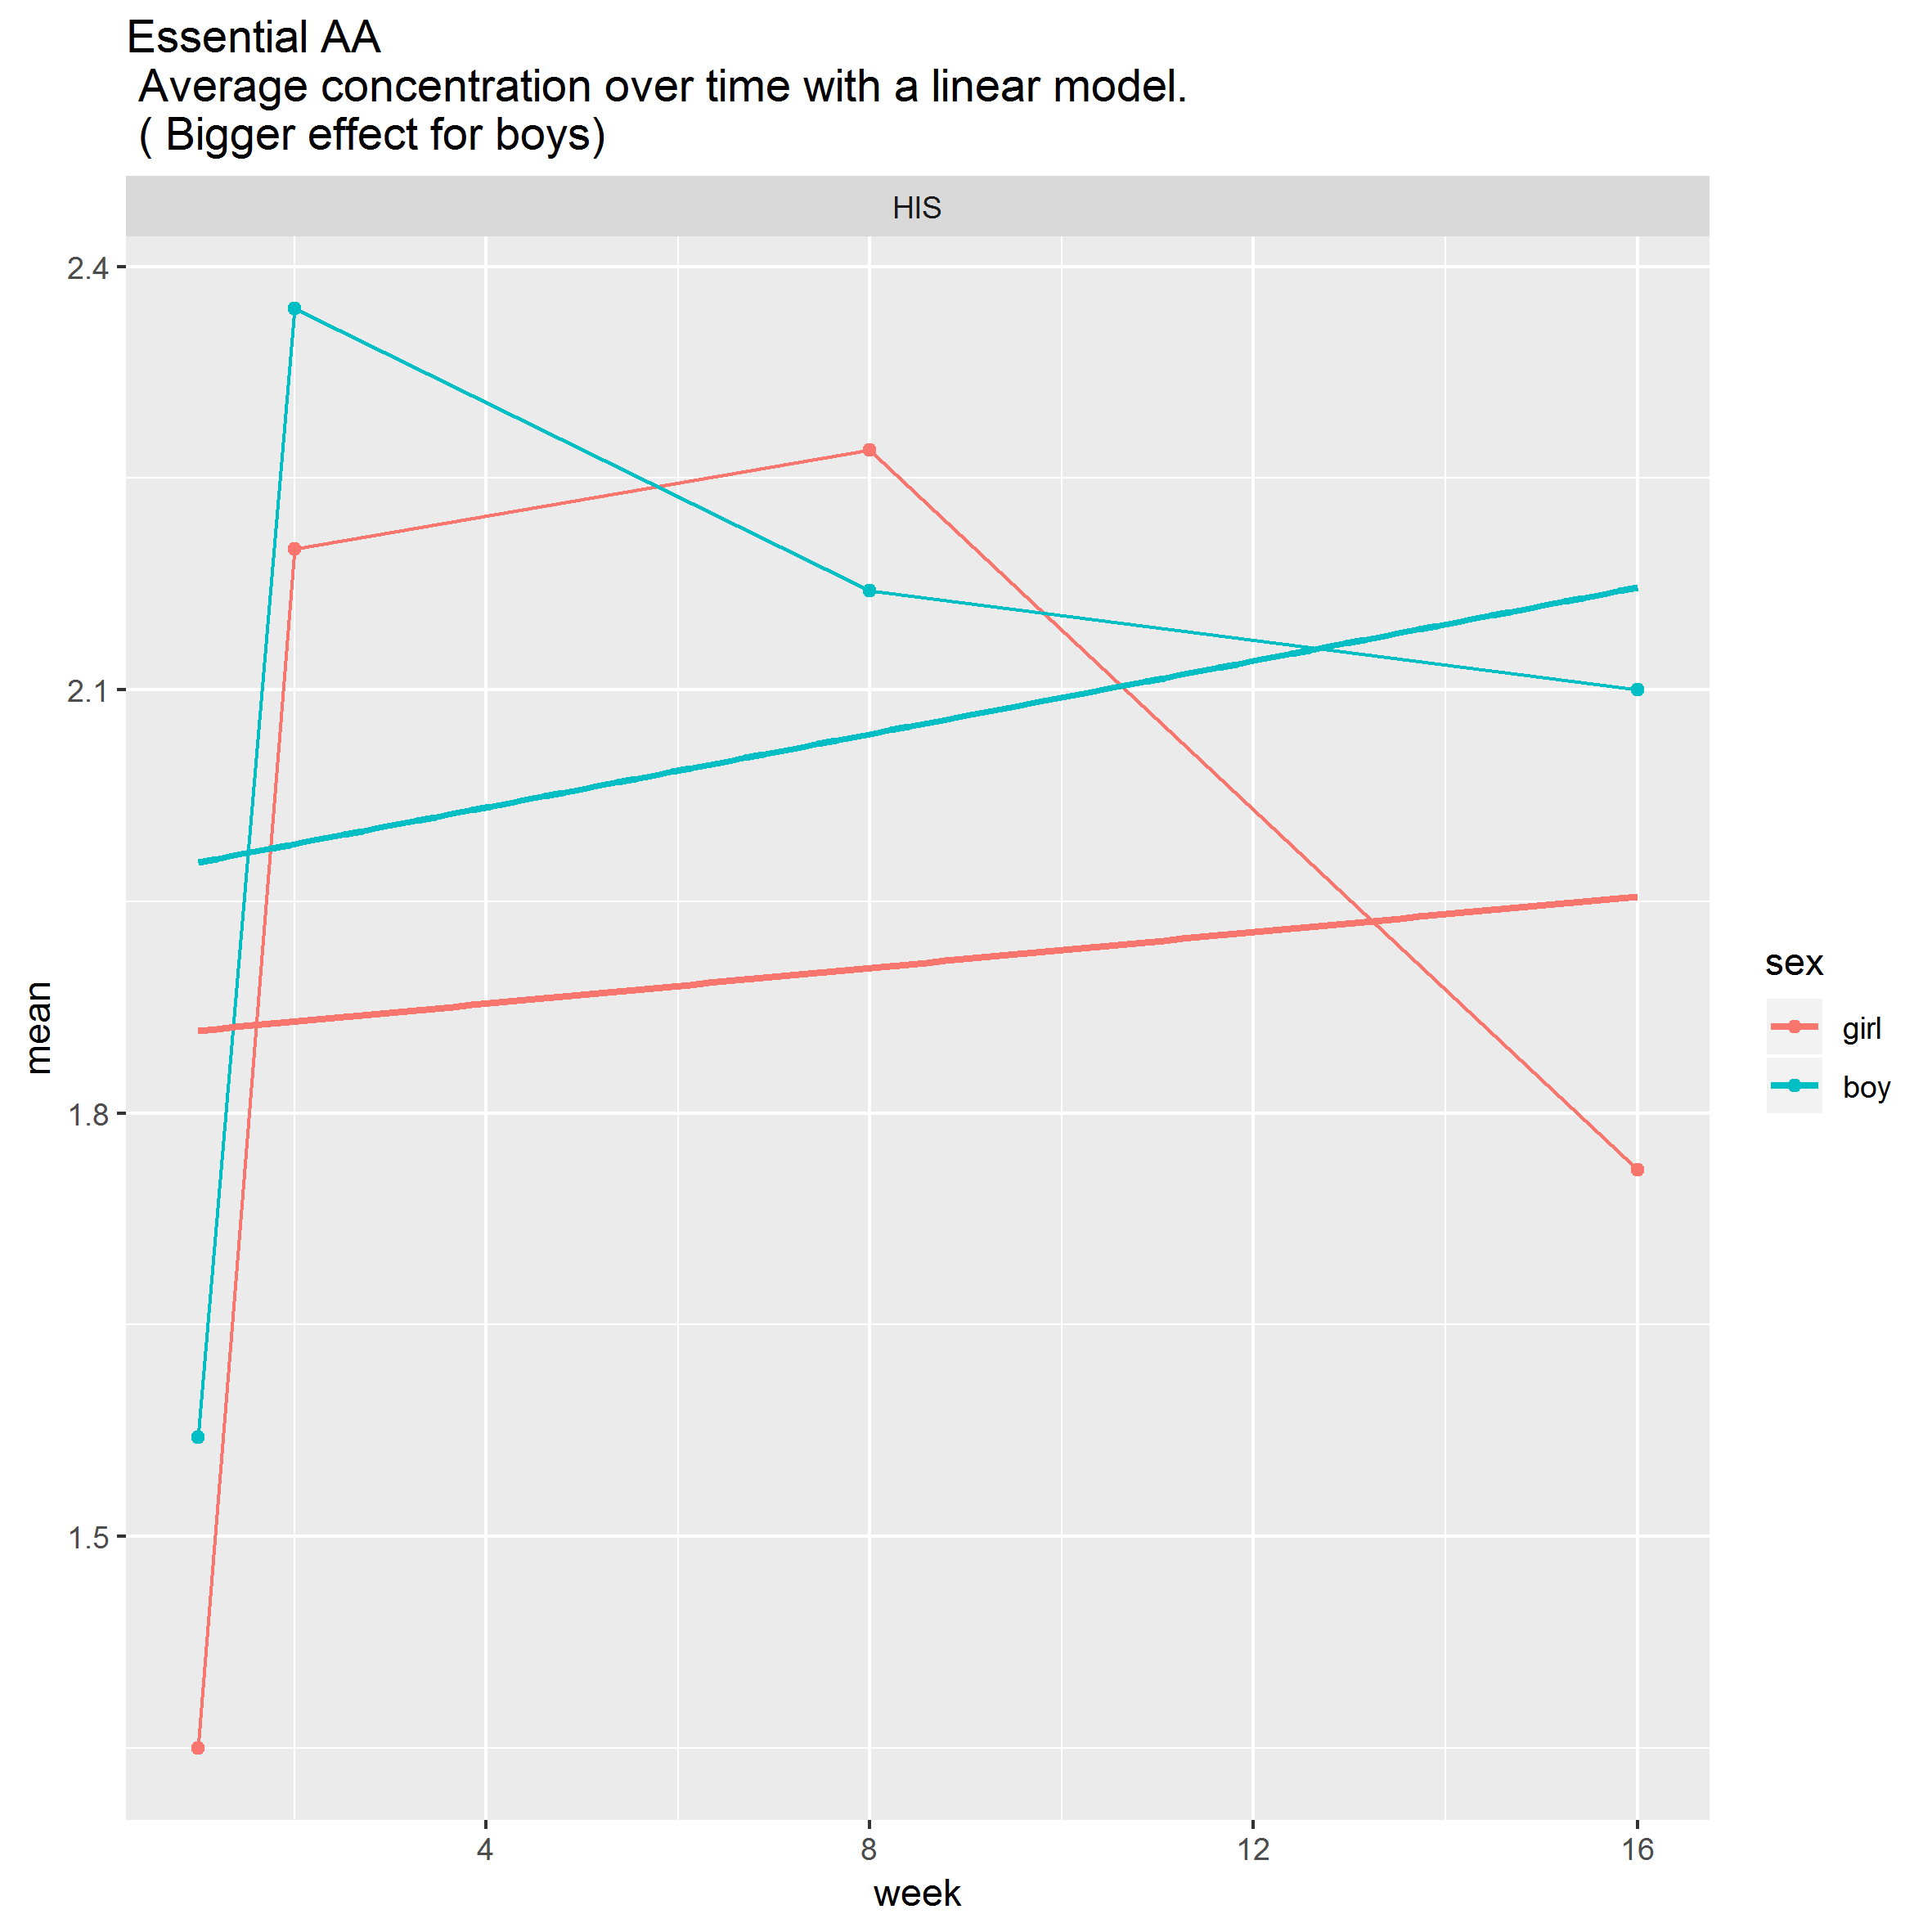
\includegraphics[width=\textwidth]{../sexweek/EAA_boys.png}
  \caption{Mean concentration per week with a linear regression line in blue for boys and pink for girls. Essential amino acids with a bigger interaction effect for boys.}
  \label{fig:EAA_boys}
\end{figure}

\begin{figure}[H]
  \centering
  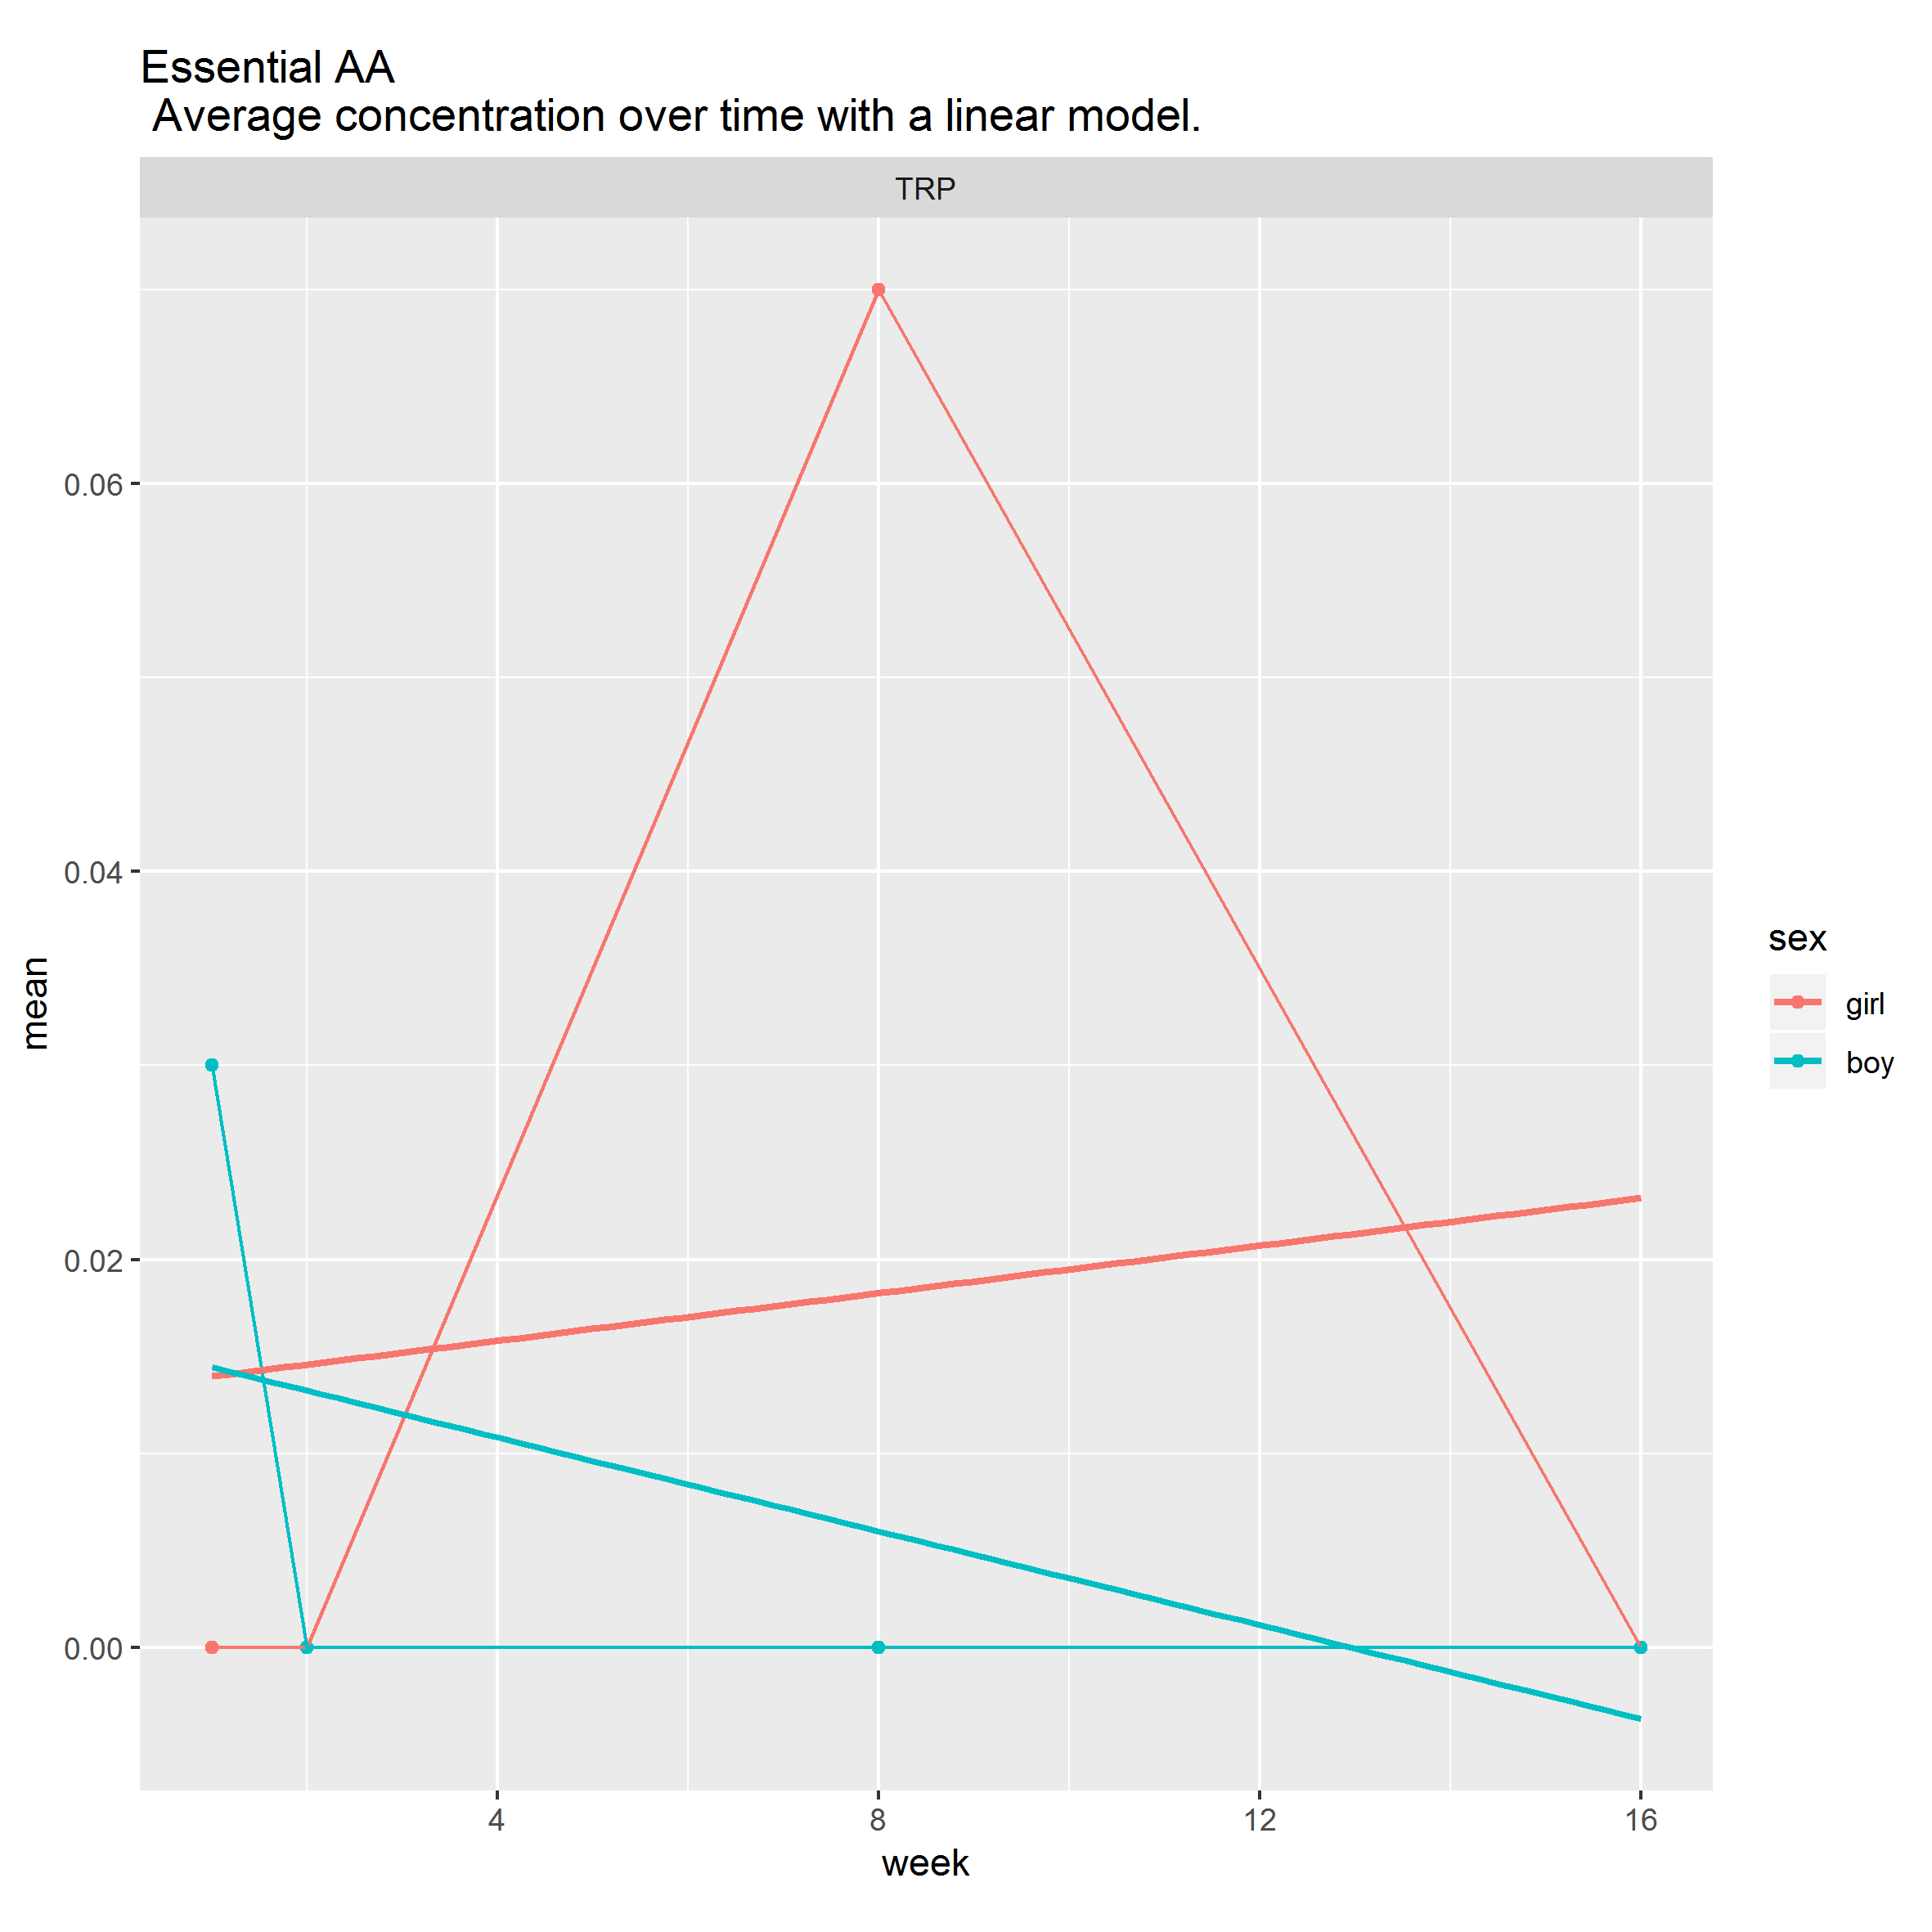
\includegraphics[width=\textwidth]{../sexweek/EAA_TRP.png}
  \caption{Mean concentration per week with a linear regression line in blue for boys and pink for girls for TRP.}
  \label{fig:EAA_TRP}
\end{figure}

\subsection{Non Essential Amino Acids}

Now, most of the effects are bigger for boys although they remain non significant. The concentration increases in a similar fashion for both sexes as can be seen in figures \ref{fig:NEAA_boys} and \ref{fig:NEAA_girls}.

In both ARG and PRO (figure \ref{fig:NEAA_girls}), the concentration for girls decreases slower mostly due to a jump in week $8$.

\begin{figure}[!htb]
  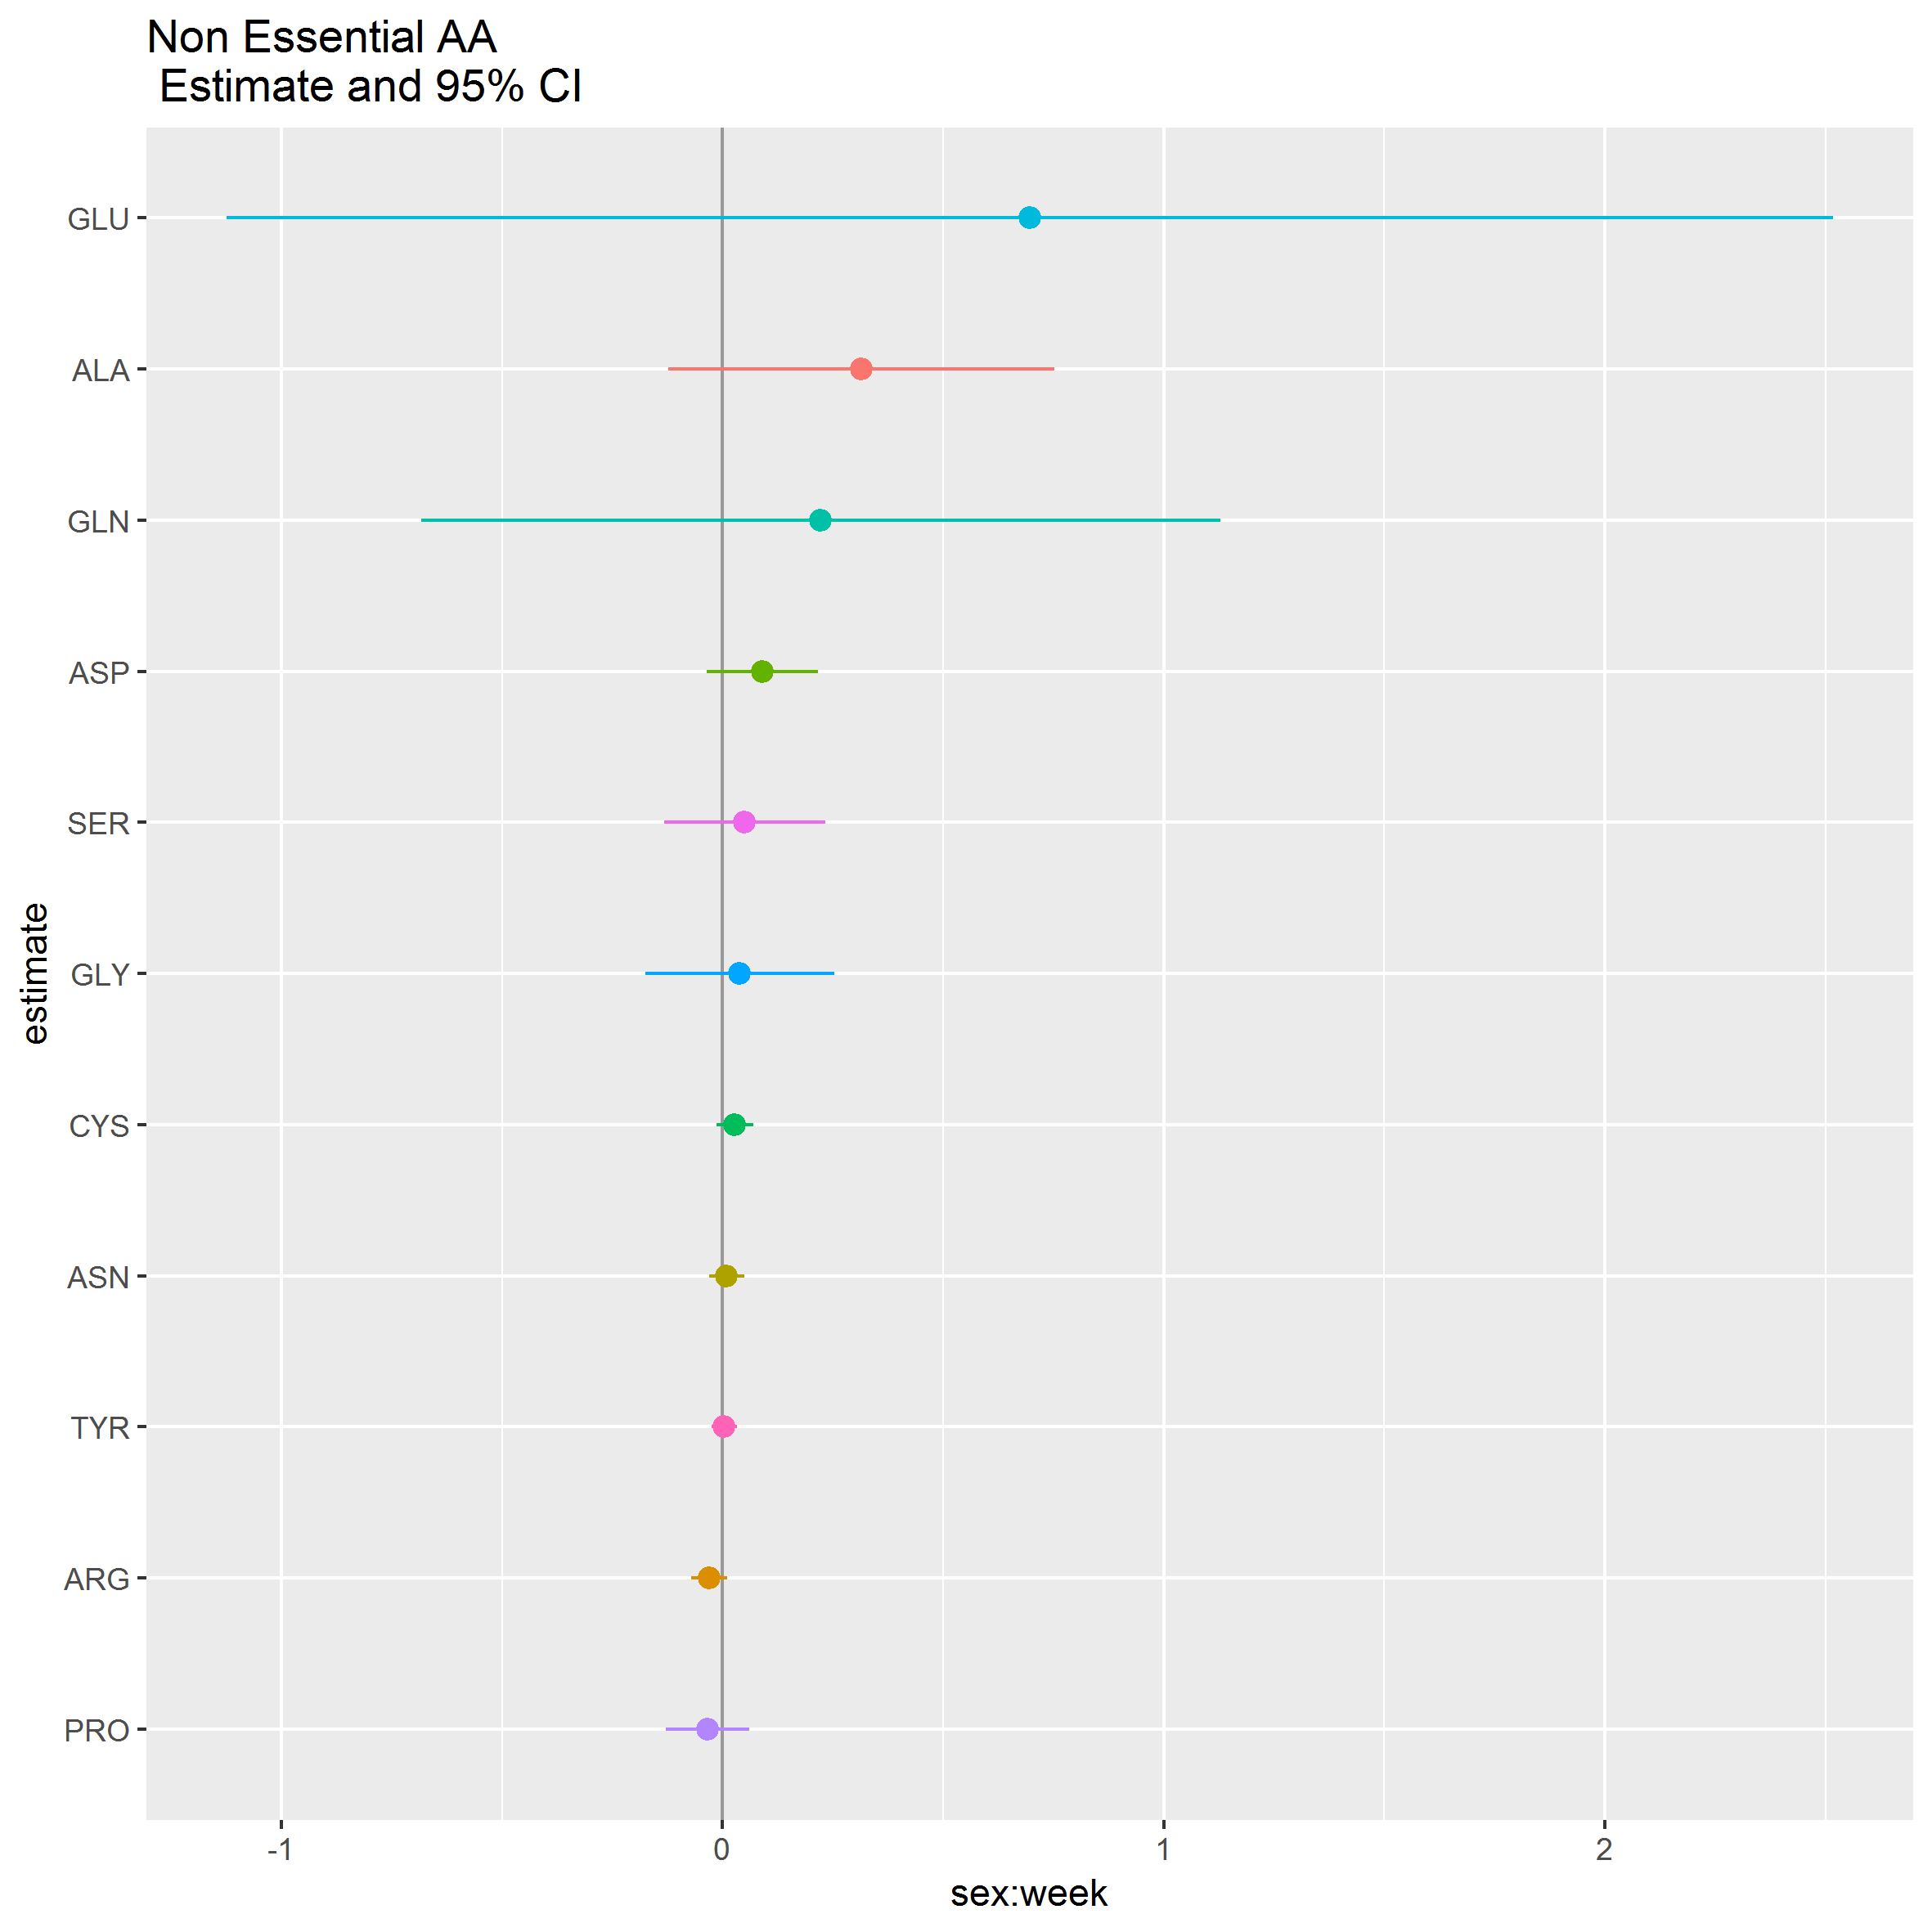
\includegraphics[width= \textwidth]{../sexweek/NEAA_SW_SW_coeff.png}
  \caption{$Sex \times week$ coefficients of model (\ref{eq:model3}) for non essential amino acids.}
  \label{fig:NEAA_SW_SW_coeff}
\end{figure}

\begin{figure}[!htb]
  \centering
  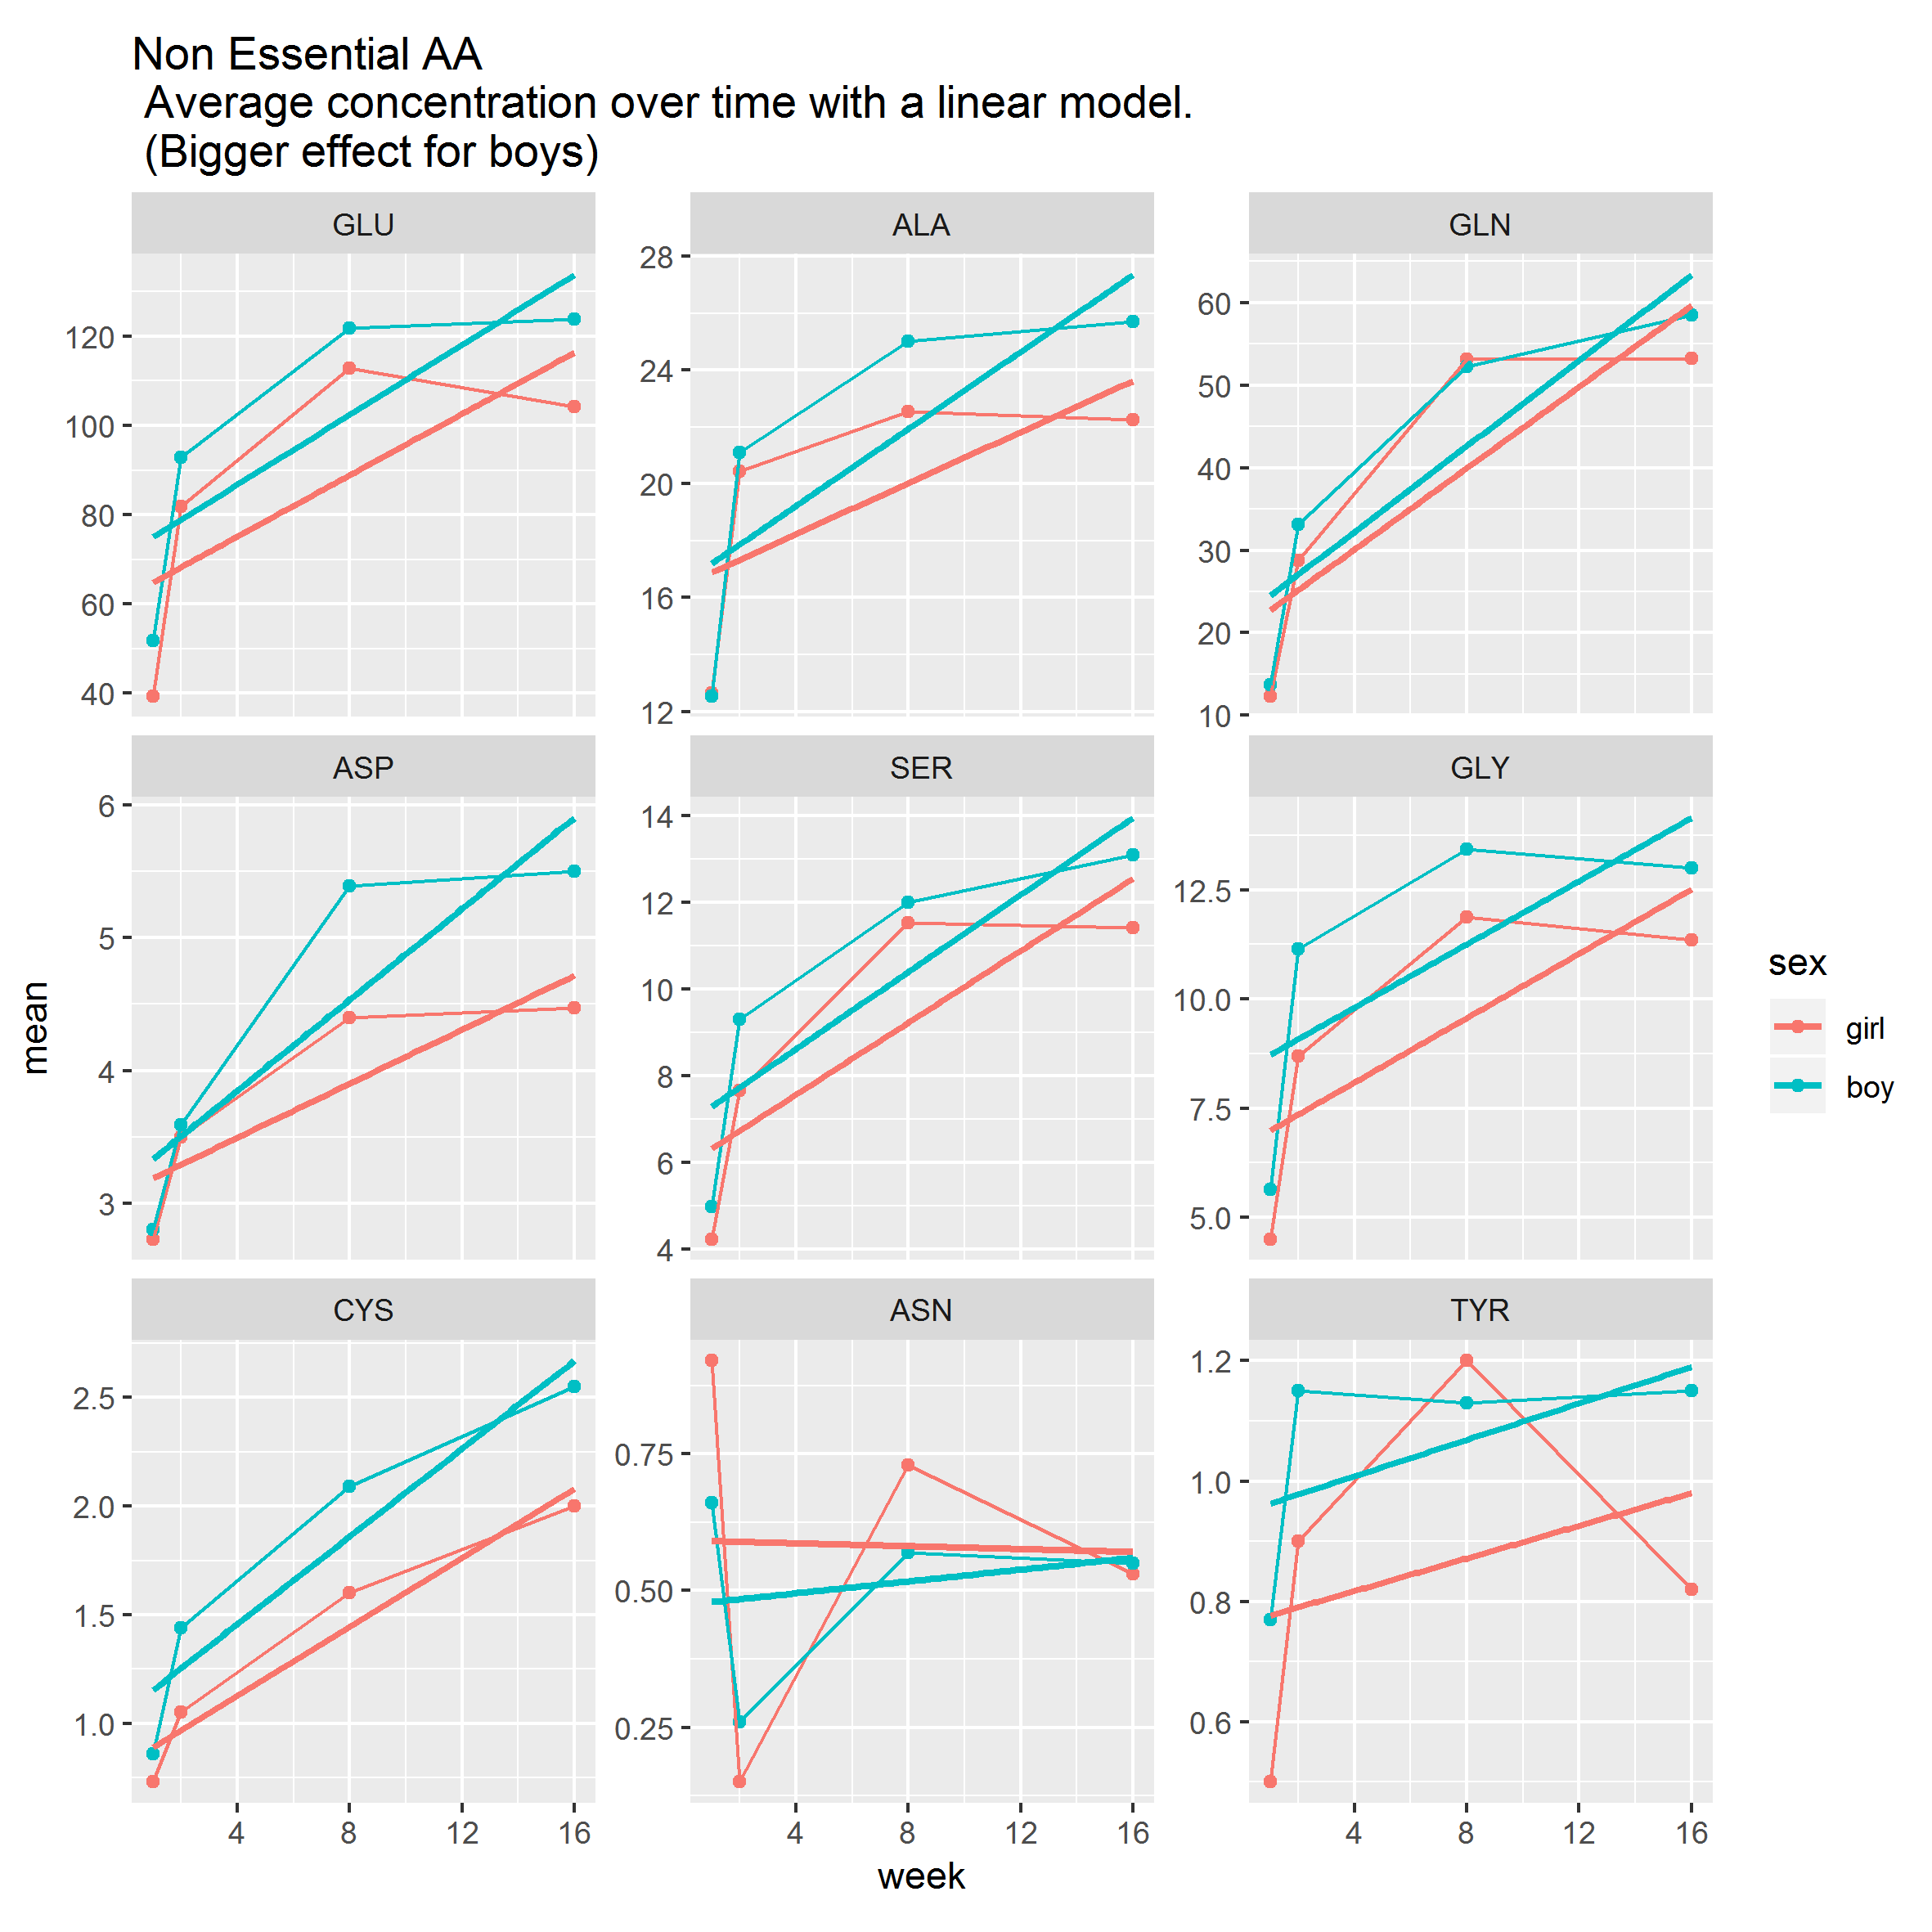
\includegraphics[width=\textwidth]{../sexweek/NEAA_boys.png}
  \caption{Mean concentration per week with a linear regression line in blue for boys and pink for girls. Non essential amino acids with a bigger interaction effect for boys.}
  \label{fig:NEAA_boys}
\end{figure}


\begin{figure}[!htb]
  \centering
  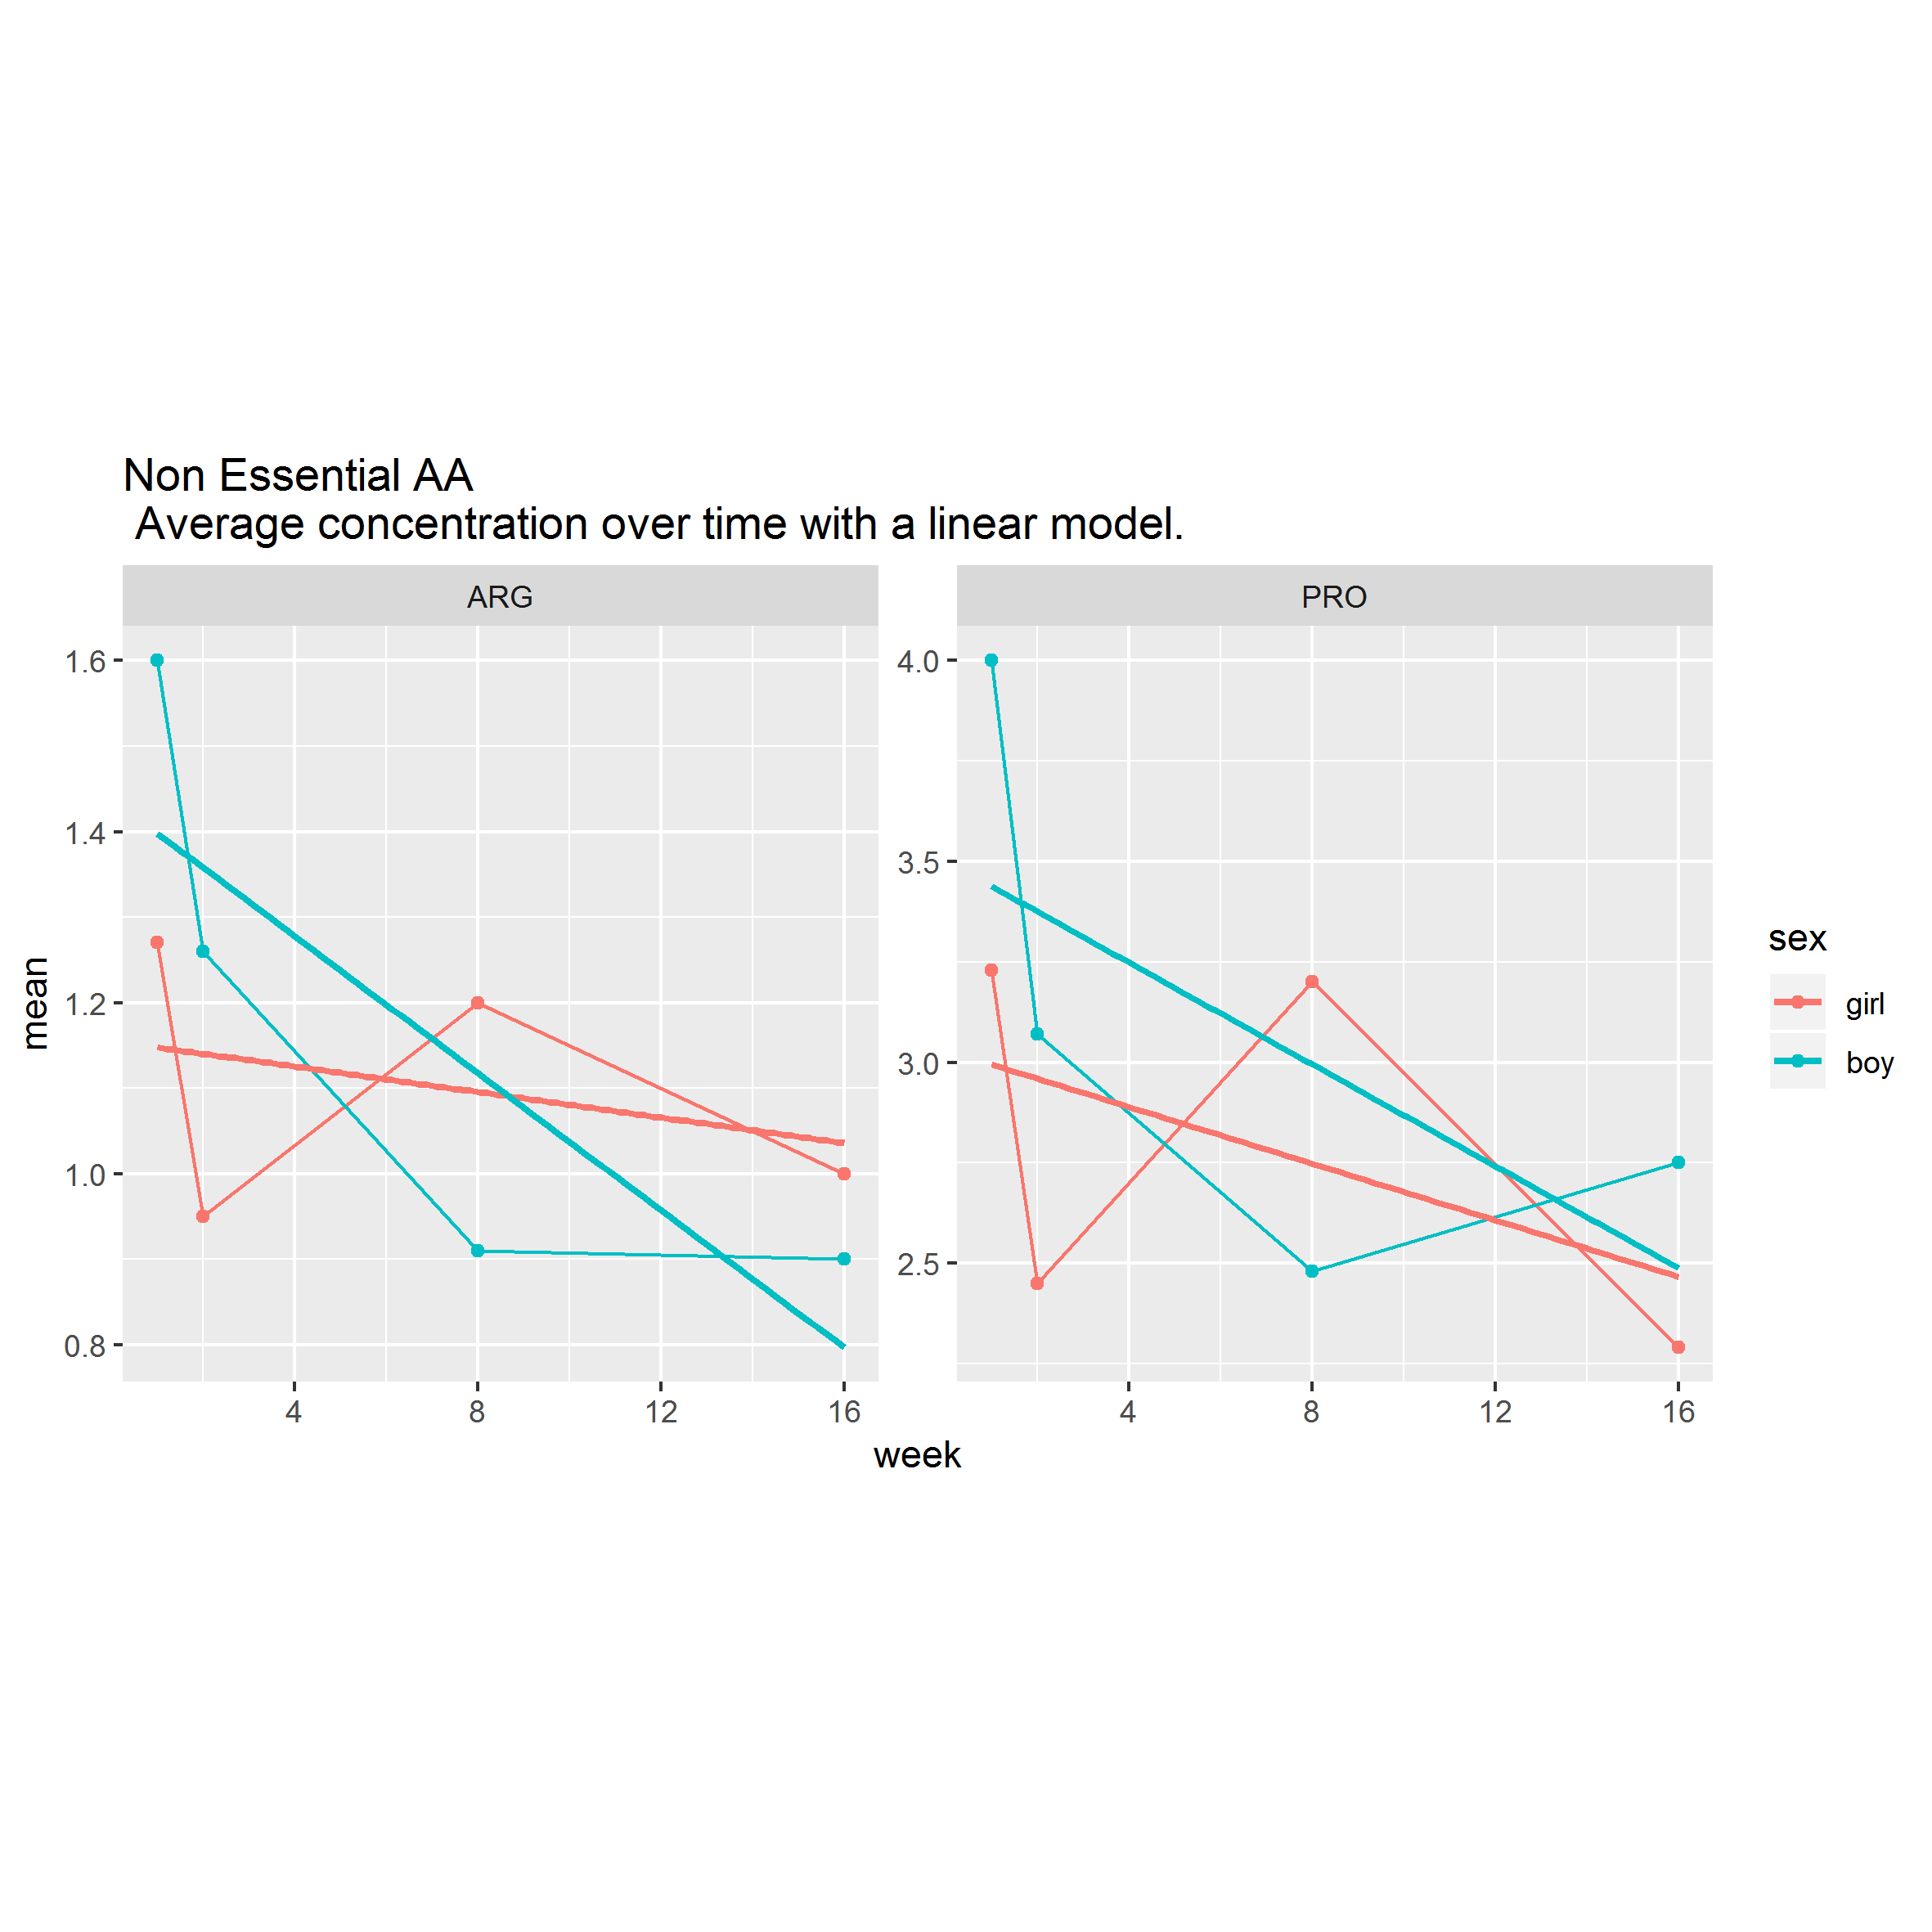
\includegraphics[width=\textwidth]{../sexweek/NEAA_girls.png}
  \caption{Mean concentration per week with a linear regression line in blue for boys and pink for girls. Non essential amino acids with a bigger interaction effect for girls.}
  \label{fig:NEAA_girls}
\end{figure}

\pagebreak

\part{What to look forward in future experiments?}

\newpage
\bibliographystyle{plain}
\bibliography{thebibliography}

\begin{thebibliography}{1}

\bibitem{NutrientsDutch} Longitudinal Variation of Amino Acid Levels in Human Milk and Their Associations with Infant Gender, Joris H. J. Van Sadelhoff, Bert J. M. Van de Heijning, Bernd Stahl, et al., Nutrients 2018, 10(9), 1233; https://doi.org/10.3390/nu10091233

%\bibitem{COBRApy} COBRApy: COnstraints-Based Reconstruction and Analysis for Python,
%Ali Ebrahim, Joshua A. Lerman, Bernhard O. Palsson, and Daniel R. Hyduke,
%BMC Systems Biology, 2013, 7:74.

\end{thebibliography}

\end{document}
